\documentclass{article}

% Language setting
\usepackage[romanian]{babel}

% Set page size and margins
% Replace `letterpaper' with`a4paper' for UK/EU standard size
\usepackage[a4paper,top=2cm,bottom=2cm,left=3cm,right=3cm,marginparwidth=1.75cm]{geometry}

% Useful packages
\usepackage{amsmath}
\usepackage{graphicx}
\usepackage[colorlinks=true, allcolors=blue]{hyperref}
\usepackage{amssymb}
\usepackage{tabto}
\usepackage{multicol}
\usepackage{hyperref}
\usepackage{mdframed}
\usepackage{xcolor}
\usepackage{mathtools}
\usepackage{wrapfig}
\usepackage{listings}

\newcommand\eqdef{\stackrel{\mathclap{\normalfont\mbox{def}}}{=}}
\newcommand\eqnot{\stackrel{\mathclap{\normalfont\mbox{not}}}{=}}
\newcommand\eqdots{\stackrel{\mathclap{\normalfont\mbox{(...)}}}{=}}

\makeatletter
\renewcommand*\env@matrix[1][c]{\hskip -\arraycolsep
  \let\@ifnextchar\new@ifnextchar
  \array{*\c@MaxMatrixCols #1}}
\makeatother

\newenvironment{mdframe16cm}{%
    \begin{mdframed}[nobreak,userdefinedwidth=16cm]
}{%
    \end{mdframed}%
}%

\hypersetup{
  colorlinks,
  citecolor=violet,
  linkcolor=black,
  urlcolor=blue}

\graphicspath{ {./images/} }

\title{Derivare si Integrare \\ Numerica}
\author{}
\date{}

\begin{document}
\maketitle

\section{Derivare}


\subsection{Introducere}

\subsubsection{Notiuni generale}
\tab Fie o functie $f:[a,b]\rightarrow\mathbb{R}$. Dorim sa calculam, in mod aproximativ, derivatele functiei $f(x)$ in anumite puncte din intervalul $[a,b]$, cunoscand valorile functiei intr-un numar redus de puncte $(x_i, f(x_i)), \, i = \overline{0, n}$.


\subsubsection{Motivatie}
\begin{itemize}
    \item In Computer Science se lucreaza in general cu date discrete si nu se cunoaste forma explicita a functiei. Astfel, trebuie aproximata valoarea derivatei in punctele de interes.
    \item Ne reamintim din capitolul de interpolare spline-urile cubice de clasa $C^2$ tensionate. Ultimele $2$ conditii necesita cunoasterea derivatelor $f'(x_0)$ si $f'(x_n)$. De cele mai multe ori, aceste valori nu se cunosc, deci trebuie aproximate.
\end{itemize} 


\subsubsection{Idee}

\begin{minipage}{0.7\textwidth}
\tabto{0.5cm} Pornim de la definita derivatei: \framebox{$f'(x_0)\; \eqdef \; $ $\displaystyle{\lim_{h \to 0}}$ $\frac{f(x_0+h)-f(x_0)}{h}$}\\

\tabto{0.5cm} Apoi, ne folosim de \textit{interpolarea Lagrange} pentru a gasi niste\\ aproximari mai bune.

\tabto{0.5cm} Vom avea in vedere si \textit{eroarea de aproximare} care intervine pe parcursul calculului.
\end{minipage}\hspace{0.75cm}
\begin{minipage}{0.3\textwidth}
    \vspace{-0.65cm}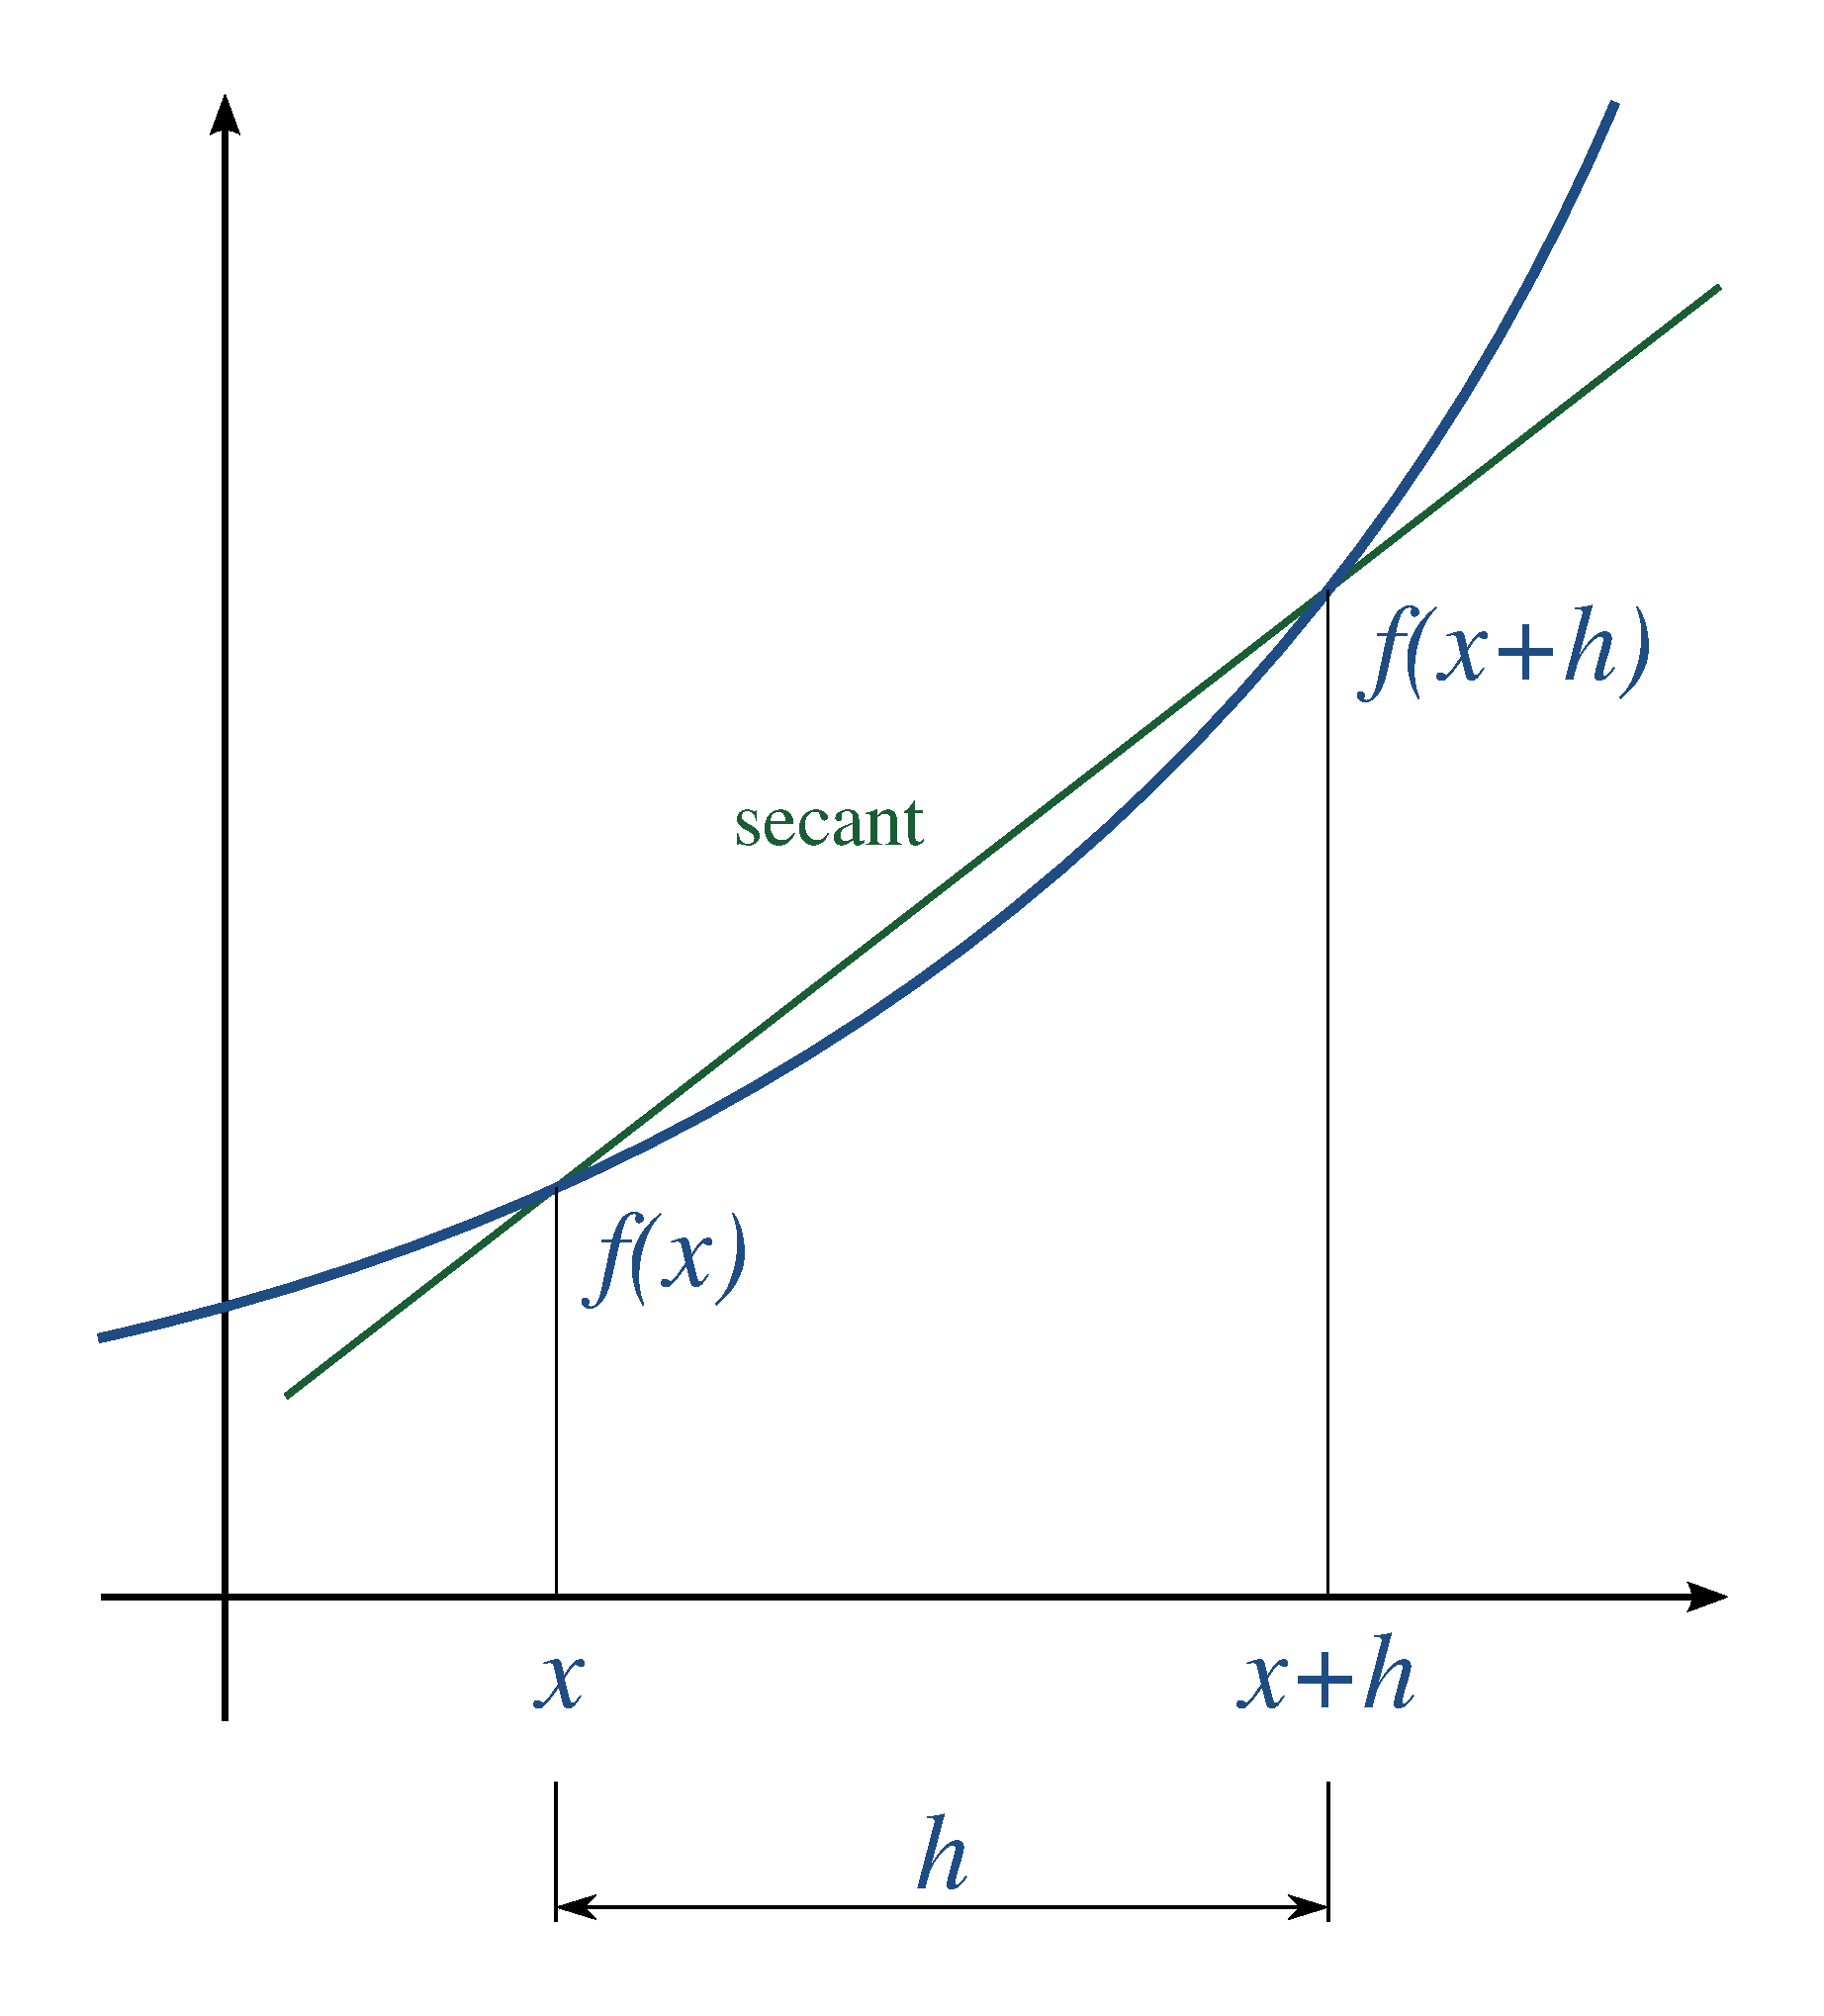
\includegraphics[scale=0.115]{derivata_limita}
\end{minipage}


\subsubsection{Moduri de aproximare abordate}
\begin{multicols}{2}
    \begin{itemize}
    
        \item Prima derivata:
        \begin{itemize}
            \item \framebox{\textbf{\hyperref[sec:two_point]{Two-Point Formulas}}}
            \item \framebox{\textbf{\hyperref[sec:three_point]{Three-Point Formulas}}}
        \end{itemize}
        
        \item A doua derivata:
        \begin{itemize}
            \item \framebox{\textbf{\hyperref[sec:sec_der]{Second Derivative Midpoint Formula}}}
            \item[]
        \end{itemize}
    
    \end{itemize}
\end{multicols}

\subsubsection{Aplicatie care foloseste derivarea numerica}
\paragraph{Edge Detection}

\tabto{0.5cm} Daca avem o \textit{imagine} si dorim sa extragem \textit{contururile} obiectelor continute in ea, trebuie sa calculam derivata imaginii\framebox[0.3cm][r]{\footnotemark}.\hspace{-0.125cm} Aceasta tehnica presupune aplicarea unui filtru (\textit{kernel}) asupra imaginii originale.
\footnotetext{\framebox[7.15cm]{\url{https://en.wikipedia.org/wiki/Image_derivatives}}}\hspace{-0.125cm} Ideea din spatele \textit{matricei de convolutie} este \textit{gradientul de imagine}\framebox[0.3cm][r]{\footnotemark}.\vspace{-0.25cm}
\footnotetext{\framebox[9.12cm]{\url{https://en.wikipedia.org/wiki/Image_gradient\#Computer_vision}}}

\tabto{0.5cm} Pentru a intelege mai bine unde este folosita derivarea numerica in cadrul procesului de extragere a contururilor, puteti viziona urmatorul clip (\textbf{Edge Detection Using Laplacian}): \href{https://www.youtube.com/watch?v=uNP6ZwQ3r6A}{
\includegraphics[scale=0.0125]{video_player}} 


\subsubsection{Pregatirea terenului}
\tab Inainte de a discutia despre fiecare mod de aproximare a derivatelor, prezentam cadrul discutiei:

\begin{itemize}
    \item Pornim de la o functie continua $f:[a,b]\rightarrow\mathbb{R}$ careia ii cunoastem valorile intr-un numar redus de puncte.
    \item Dorim sa gasim o aproximatie cat mai buna pentru valorile derivatelor functiei $f(x)$.
\end{itemize}


\subsubsection{Estimarea erorii interpolarii polinomiale}
\label{sec:est_err}
\tab Fie $f(x)$ cu $x \in [a,b]$ si un suport al interpolarii $S=[(x_0, f(x_0)), (x_1, f(x_1)),\dots,(x_n, f(x_n))]$.\vspace{0.1cm}

Fie $P_n(x)$ polinomul de grad $n$ care \textit{interpoleaza} functia $f(x)$ pe $[a,b]$, adica $P_n(x_i) = f(x_i), \forall~\,~i~=~\overline{0, n}$.

\textbf{Functia eroare}\framebox[0.3cm][r]{\footnotemark} se defineste astfel:
\framebox{$\textcolor{red}{e(x)} = f(x) - P(x)$}, $x \in [a,b]$ si
$\begin{cases}
    f(x) = valoarea\; reala\\
    P_n(x) = valoarea\; aproximata
\end{cases}$
\footnotetext{\framebox[11.25cm]{\url{https://en.wikipedia.org/wiki/Polynomial_interpolation\#Interpolation_error}}}

De acum inainte, tot ce este marcat cu \textcolor{red}{rosu}, face parte din termenii \textit{erorii de aproximatie}.\vspace{0.25cm}

\textbf{Teorema:}
Fie $f(x)$ o functie de clasa $C^{n+1}$ pe intervalul $[a,b]$ si $P_n(x)$ un polinom de grad cel mult $n$ care interpoleaza functia $f$ in $n+1$ puncte distincte din $[a,b]$.
Atunci, pentru orice $x \in [a,b]$, exista un punct $\xi_x \in [a,b]$, astfel incat eroare de aproximare se poate exprima.

Matematic, aceasta are forma:
\framebox{$\textcolor{red}{e(x)} = \frac{1}{(n+1)!} \cdot f^{(n+1)}(\xi_x) \cdot \prod\limits_{\substack{i=0}}^{n} (x-x_i)$}


\subsection{Prima derivata}
\tab Asa cum am vazut in capitolul de interpolare, polinoamele au avantajul ca se pot deriva (si integra) foarte usor.
Asadar, putem gasi niste aproximari ale derivatei $f'(x)$, ajutandu-ne de o tehnica de interpolare.

Inainte de a prezenta moduri de aproximare ale derivatei, reamintim faptul ca atunci cand gradul polinomului de interpolare este mare, apar oscilatii in capete si eroarea de aproximare creste foarte mult. 

Deci, trebuie sa mentinem gradul polinomului de interpolare mic. In cele ce urmeaza, vom trata cazurile in care suportul interpolarii este format din $2$ sau $3$ puncte.


\subsubsection{2 puncte (n=1)}
\label{sec:two_point}

\paragraph{Modul de determinare}

\tabto{0.5cm} Inainte de toate, pentru a aproxima $f'(x_0)$, facem ipotezele:
$\begin{cases}
    x_0 \in (a,b) \\
    f \in C^2[a,b] \\
    x_1=x_0+h,\; $cu $h$ suficient de mic, a.\^{i}. $x_1 \in (a,b)$ $\\
\end{cases}$\\

Asadar, suportul interpolarii arata astfel:
$S = [(x_0, f(x_0)), (x_1, f(x_1))]$

Aproximam functia $f(x)$ cu ajutorul polinomului de interpolare \textit{Lagrange} (de grad $n=1$):

$f(x) \simeq P_1(x)$, $x \in (x_0, x_1)$ (Punem conditia ca $x$ sa se afle intre $x_0$ si $x_1$ pentru ca interpolarea facuta are \textit{valabilitate}\framebox[0.3cm][r]{\footnotemark} doar intre cele 2 puncte $\equiv$ doar in suportul interpolarii)\\
\footnotetext{\framebox[6.15cm]{\url{https://stats.stackexchange.com/a/418898}}}

Interpoland Lagrange intre punctele $x_0$ si $x_1$, obtinem:
$P_1(x) = f(x_0) \cdot \frac{x-x_1}{x_0-x_1} + f(x_1) \cdot \frac{x-x_0}{x_1-x_0}$

Derivam expresia obtinuta:
$P_1'(x) = f(x_0) \cdot \frac{1}{x_0-x_1} + f(x_1) \cdot \frac{1}{x_1-x_0}$

Tinem cont de faptul ca $x_1 = x_0+h$ (ipoteza initiala) si substituim in expresia de mai sus.

Astfel, gasim ca: $P_1'(x) = f(x_0) \cdot \frac{-1}{h} + f(x_0+h) \cdot \frac{1}{h} \iff$ \framebox{$P_1'(x) = \frac{f(x_0+h) - f(x_0)}{h}$}\\

Pornim de la functia eroare \framebox{$\textcolor{red}{e(x)} = f(x) - P_1(x)$} si ne folosim de \textit{\hyperref[sec:est_err]{teorema prezentata anterior}}:

$f(x) = P_1(x) + \textcolor{red}{\frac{1}{2!} \cdot f''(\xi(x)) \cdot (x-x_0)(x-x_1)} \; |()'$
$\Rightarrow f'(x) = P_1'(x) + \textcolor{red}{\frac{d}{dx}[\frac{(x-x_0)(x-x_1)}{2} \cdot f''(\xi(x))]}$\vspace{0.15cm}

Dar, $P_1'(x) = \frac{f(x_0+h)-f(x_0)}{h}$ (reamintim ca $x_1=x_0+h$)
$\Rightarrow f'(x) = \frac{f(x_0+h)-f(x_0)}{h} + \textcolor{red}{\frac{d}{dx}[\frac{(x-x_0)(x-x_0-h)}{2} \cdot f''(\xi(x))]}$\vspace{0.15cm}

$\Rightarrow$ \framebox{$f'(x) = \frac{f(x_0+h)-f(x_0)}{h} + \textcolor{red}{\frac{2(x-x_0)-h}{2} \cdot f''(\xi(x)) + \frac{(x-x_0)(x-x_0-h)}{2} \cdot \frac{d}{dx}[f''(\xi(x))]}$} \textbf{(1)}\\

Eliminand termenii care contin expresia $\xi(x)$ (termenii scrisi cu \textcolor{red}{rosu}), obtinem urmatoarea aproximatie:
\framebox{$f'(x) \simeq \frac{f(x_0+h)-f(x_0)}{h},\; \forall x \in [x_0, x_0+h]$}\\

O problema cu formula \textbf{(1)} este ca nu avem informatii despre $\frac{d}{dx}[f''(\xi(x))]$ si astfel nu putem sa estimam eroarea de aproximare.

Dar, cand facem $x=x_0$, coeficientul lui $\frac{d}{dx}[f''(\xi(x))]$ devine $0$ si formula se reduce la:

\begin{mdframe16cm}
\paragraph{Two-Point Formula}\vspace{-0.25cm}
\tabto{0.5cm}\framebox{$f'(x_0) = \frac{f(x_0+h)-f(x_0)}{h} - \textcolor{red}{\frac{h}{2} \cdot f''(\xi)}$} ($\xi$ se afla intre $x_0$ si $x_0+h$) \textbf{(*)}\\
\end{mdframe16cm}


Formula \textbf{(*)} este o metoda de \textbf{ordin 1\hspace{0.05cm}}\framebox[0.3cm][r]{\footnotemark} si poarta denumirile:
$\begin{cases}
    $\textbf{forward-difference formula}$,\; h > 0 \\
    $\textbf{backward-difference formula}$,\; h < 0 \\
\end{cases}$\\
\footnotetext{\framebox[7.2cm]{\url{https://en.wikipedia.org/wiki/Order_of_accuracy}}}

Pentru \textit{valori mici} ale lui $h$, aproximatia $f'(x_0) \simeq \frac{f(x_0+h)-f(x_0)}{h}$ se face cu o eroare de ordinul $M \cdot  \frac{|h|}{2}$, unde $M$ este maximul atins de functia $|f''(\xi(x))|$ pe intervalul $[x_0, x_0+h]$.\vspace{0.15cm}

\paragraph{Exemplu numeric}

\tabto{0.5cm} Fie functia $f(x) = ln(x)$. Aproximati $f'(1.8)$ folosind, pe rand, pasul 
$\begin{cases}
    h = 0.1 \\
    h = 0.05 \\
    h = 0.01
\end{cases}$\vspace{-0.5cm}

Determinati si limitele erorii de aproximare.\\

Folosim \textit{forward-difference formula}: $f'(x_0) \simeq \frac{f(x_0+h)-f(x_0)}{h} \iff f'(1.8) \simeq \frac{f(1.8+h)-f(1.8)}{h}$\\

Prezentam rezolvarea completa pentru pasul $h=0.1$:\vspace{0.1cm}

$f'(1.8) \simeq \frac{f(1.8+0.1)-f(1.8)}{0.1} \iff f'(1.8) \simeq \frac{ln(1.9)-ln(1.8)}{0.1} \iff$ \framebox{$f'(1.8) \simeq 0.5406722$}\\

Pentru limitele erorii de aproximare, avem: $f''(x) = -\frac{1}{x^2}$ si $1.8 < \xi < 1.9 \xRightarrow[]{\textbf{(*)}}$

$\Rightarrow err_{h=0.1} = \frac{|h \cdot f''(\xi)|}{2} = \frac{|h|}{2 \xi^2} < \frac{0.1}{2 \cdot (1.8)^2} \Rightarrow$
\framebox{\textcolor{red}{$err_{h=0.1} < 0.0154321$}}\\

\begin{minipage}{0.55\textwidth}
Analog se procedeaza si pentru $h=0.05$ si $h=0.01$

Rezultatele sunt prezentate in tabelul alaturat:
\end{minipage}
\begin{minipage}{0.45\textwidth}
    \begin{tabular}{c | c | c}
        Pasul & Aproximatia & \textcolor{red}{Limita erorii} \\
        \hline
        \rule{0pt}{1\normalbaselineskip}h & $\frac{f(1.8+h)-f(1.8)}{h}$ & $\frac{|h|}{2\cdot (1.8)^2}$ \\
        \hline
        0.1  & 0.5406722 & 0.0154321 \\
        \hline
        0.05 & 0.5479795 & 0.0077160 \\
        \hline
        0.01 & 0.5540180 & 0.0015432 \\
    \end{tabular}
\end{minipage}\\

\tabto{0.5cm} Derivata functiei $f(x) = ln(x)$ este $f'(x) = \frac{1}{x},\; \forall x > 0$, deci valoarea exacta a derivatei functiei $f(x)$ in punctul $1.8$ este $f'(1.8) = \frac{1}{1.8} = 0.55\overline{5}$. In acest caz, am obtinut aproximatii foarte bune, chiar si cu cel mai mare pas. Insa, cu cat pasul $h$ este mai mic, cu atat vom obtine aproximatii mai bune.\\

\begin{minipage}{0.4\textwidth}
    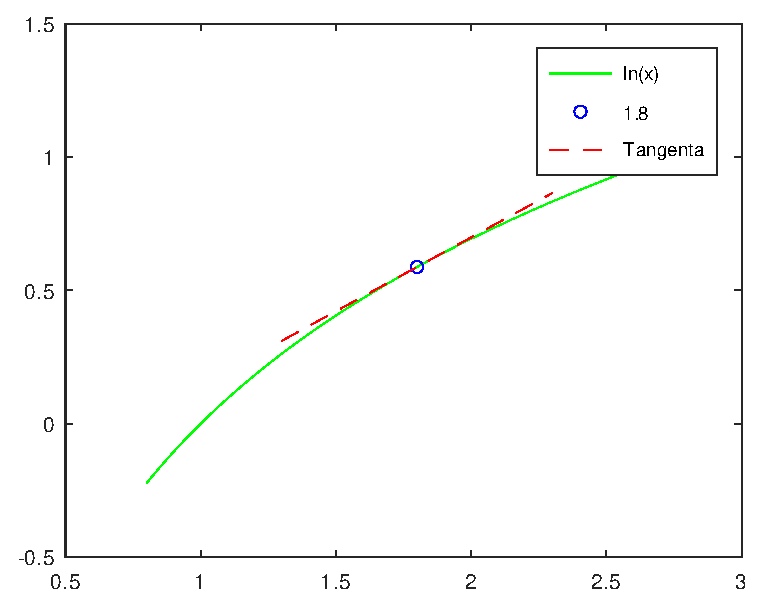
\includegraphics[scale=0.45]{two_points_ex}
\end{minipage}
{\LARGE$\xrightarrow[]{Zoom}$}\;\;\;\;\;
\begin{minipage}{0.65\textwidth}
    \framebox{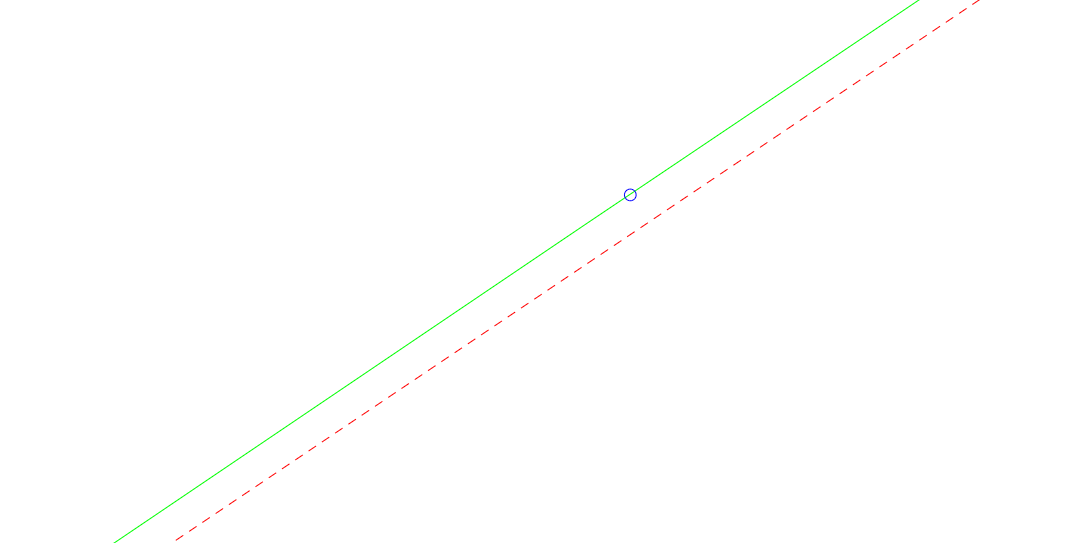
\includegraphics[scale=0.3]{two_points_zoom}}
\end{minipage}

\paragraph{Ce putem imbunatati?}

\tabto{0.5cm} Pana acum, am lucrat cu $2$ puncte in suportul interpolarii. Teoretic, cu cat avem mai multe informatii, cu atat putem sa aproximam mai bine. In continuare, ne indreptam atentia catre formule de aproximare care implica $3$ puncte in suportul de interpolare.


\subsubsection{3 puncte (n=2)}
\label{sec:three_point}

\paragraph{Modul de determinare}

\tabto{0.5cm} In cele ce urmeaza, lucram cu $3$ puncte in suportul interpolarii. Formulele pe care le vom deduce sunt foarte utile daca cele $3$ puncte sunt \textit{echidistante}.

Asadar, vom considera:
$\begin{cases}
    x_0 = x_0 \\
    x_1 = x_0 + h \\
    x_2 = x_0 + 2h \\
\end{cases} (h \neq 0)$\\

Modeland putin \textit{\hyperref[sec:est_err]{teorema privind estimarea erorii}}, obtinem urmatoarea formula \textit{generala} de aproximare a derivatei I: 

\framebox{$f'(x_j) = \sum\limits_{k=0}^{n} f(x_k) L'_k(x_j) + \textcolor{red}{\frac{f^{(n+1)}(\xi(x_j))}{(n+1)!} \prod\limits_{\substack{k=0 \\ k \neq j}}^{n} (x_j-x_k)}$} (s.n. \textbf{(n+1)-point formula})\\

In general, folosind mai multe puncte pentru a aproxima $f'(x_j)$ in ecuatia dedusa anterior, vom obtine o acuratete mai mare, cu toate ca pentru un numar mare de evaluari (multe puncte), eroarea de rotunjire\framebox[0.3cm][r]{\footnotemark} creste.
\footnotetext{\framebox[3.5cm]{\url{https://bit.ly/3k1hJas}}}

\textit{Observatie:} Cele mai utilizate formule sunt cele care implica $1$, $3$ sau $5$ puncte. In continuare, vom trata cazul cu $3$ puncte:\vspace{-0.5cm}

\tabto{0.5cm} Inainte de toate, pentru a aproxima $f'(x_0)$, facem ipotezele:
$\begin{cases}
    x_0 \in (a,b) \\
    f \in C^2[a,b] \\
    x_1=x_0+h,\; $cu $h$ suficient de mic, a.\^{i}. $x_1 \in (a,b)$ $\\
    x_2=x_0+2h,\; $cu $h$ suficient de mic, a.\^{i}. $x_2 \in (a,b)$ $
\end{cases}$\\

Asadar, suportul interpolarii arata astfel:
$S = [(x_0, f(x_0)), (x_1, f(x_1)), (x_2, f(x_2))]$

Aproximam functia $f(x)$ cu ajutorul polinomului de interpolare \textit{Lagrange} (de grad $n=2$):

$f(x) \simeq P_2(x)$ cu $x \in (x_0, x_2)$ si
$P_2(x) = f(x_0) \cdot L_0(x) + f(x_1) \cdot L_1(x) + f(x_2) \cdot L_2(x)$ \\

Pornim de la \textit{multiplicatorii Lagrange}:
$\begin{cases}
    L_0(x) = \frac{(x-x_1)(x-x_2)}{(x_0-x_1)(x_0-x_2)} \vspace{0.15cm}\\
    L_1(x) = \frac{(x-x_0)(x-x_2)}{(x_1-x_0)(x_1-x_2)} \vspace{0.15cm}\\
    L_2(x) = \frac{(x-x_0)(x-x_1)}{(x_2-x_0)(x_2-x_1)} \\
\end{cases}$
$\xRightarrow[]{\textbf{()'}}$
$\begin{cases}
    L_0'(x) = \frac{2x-x_1-x_2}{(x_0-x_1)(x_0-x_2)} \vspace{0.15cm}\\
    L_1'(x) = \frac{2x-x_0-x_2}{(x_1-x_0)(x_1-x_2)} \vspace{0.15cm}\\
    L_2'(x) = \frac{2x-x_0-x_1}{(x_2-x_0)(x_2-x_1)} \\
\end{cases}$\\

Derivand polinomul de interpolare Lagrange, obtinem:

$P_2'(x) = f(x_0) \cdot L_0'(x) + f(x_1) \cdot L_1'(x) + f(x_2) \cdot L_2'(x)$\\

Particularizam \textbf{(n+1)-point formula} pentru $n=2$:

$f'(x_j) = f(x_0) \cdot [\frac{2x-x_1-x_2}{(x_0-x_1)(x_0-x_2)}] + f(x_1) \cdot [\frac{2x-x_0-x_2}{(x_1-x_0)(x_1-x_2)}] + f(x_2) \cdot [\frac{2x-x_0-x_1}{(x_2-x_0)(x_2-x_1)}] + \textcolor{red}{\frac{f^{(3)}(\xi_j)}{3!} \prod\limits_{\substack{k=0 \\ k \neq j}}^{2} (x_j-x_k)}$\\

Am obtinut formula generala pentru $3$ puncte in suportul interpolarii.

Reamintim ipotezele legate de puncte ($x_j=x_0,\; x_1=x_0+h$ si $x_2=x_0+2h$) si substituim in expresia obtinuta anterior.
\framebox{$f'(x_0) = \frac{1}{h} [-\frac{3}{2}f(x_0) + 2f(x_0+h) -\frac{1}{2}f(x_0+2h)] + \textcolor{red}{\frac{h^2}{3}f^{(3)}(\xi_0)}$}\\

Analog pentru $x_j=x_1$: \framebox{$f'(x_0+h) = \frac{1}{h} [-\frac{1}{2}f(x_0) + \frac{1}{2}f(x_0+2h)] - \textcolor{red}{\frac{h^2}{6}f^{(3)}(\xi_1)}$}\\

Analog pentru $x_j=x_2$: \framebox{$f'(x_0+2h) = \frac{1}{h} [\frac{1}{2}f(x_0) - 2f(x_0+h) + \frac{3}{2}f(x_0+2h)] + \textcolor{red}{\frac{h^2}{3}f^{(3)}(\xi_2)}$}\\

In a doua ecuatie, se face schimbarea de variabila $x_0+h \rightarrow x_0$, pentru a determina o aproximare a derivatei in punctul $x_0$. Analog in ultima ecuatie: $x_0+2h \rightarrow x_0$.\\

In final, se obtin urmatoarele $3$ formule:
$\begin{cases}
    \vspace{0.1cm}f'(x_0) = \frac{1}{2h}[-3f(x_0) + 4f(x_0+h) - f(x_0+2h)] + \textcolor{red}{\frac{h^2}{3}f^{(3)}(\xi_0)} \\
    \vspace{0.1cm}f'(x_0) = \frac{1}{2h}[-f(x_0-h) + f(x_0+h)] - \textcolor{red}{\frac{h^2}{6}f^{(3)}(\xi_1)} \\
    f'(x_0) = \frac{1}{2h}[f(x_0-2h) - 4f(x_0-h) + 3f(x_0)] +\textcolor{red}{\frac{h^2}{3}f^{(3)}(\xi_2)}
\end{cases}$\\

Este usor de observat ca daca substituim $h$ cu $-h$ in prima ecuatie, obtinem ultima ecuatie. \newpage

Practic, raman doar $2$ formule:

\begin{mdframe16cm}\vspace{-0.25cm}
\paragraph{Three-Point Endpoint Formula}

\tabto{0.5cm}\framebox{$f'(x_0) = \frac{1}{2h}[-3f(x_0) + 4f(x_0+h) - f(x_0+2h)] + \textcolor{red}{\frac{h^2}{3}f^{(3)}(\xi)}$} ($\xi$ se afla intre $x_0$ si $x_0+2h$)~\textbf{(**)}
\end{mdframe16cm}

\begin{mdframe16cm}\vspace{-0.25cm}
\paragraph{Three-Point Midpoint Formula}
\tabto{0.5cm}\framebox{$f'(x_0) = \frac{1}{2h}[f(x_0+h) - f(x_0-h)] - \textcolor{red}{\frac{h^2}{6}f^{(3)}(\xi)}$} ($\xi$ se afla intre $x_0-h$ si $x_0+h$) \textbf{(***)}\\ 
\end{mdframe16cm}

Cu toate ca ambele formule \textbf{(**)} si \textbf{(***)} sunt metode de \textbf{ordin 2}, eroarea din ecuatia (***) este aproximativ \textit{jumatate} din eroarea provenita in ecuatia (**), deoarece formula (***) foloseste informatii din ambele parti ale punctului $x_0$, pe cand (**) foloseste puncte doar dintr-o parte.\\

\textit{Observatie:} Ecuatia (**) se dovedeste ceva mai utila atunci cand se doreste aproximarea derivatei in apropierea capetelor intervalului, deoarece informatii despre functia $f$ in afara intervalului, de obicei, nu sunt cunoscute.

\paragraph{Exemplu numeric}

\begin{align*}
    \tabto{0.5cm}\begin{minipage}{0.4\textwidth}
    \tabto{0.5cm} Fie functia $f(x) = xe^x$. Aproximati $f'(2)$, cunoscand urmatorul suport de interpolare:
    \end{minipage}\hspace{1cm}
    \begin{minipage}{0.4\textwidth}
        \begin{tabular}{c | c}
            x & f(x) \\
            \hline
            1.8 & 10.889365 \\
            \hline
            1.9 & 12.703199 \\
            \hline
            \textbf{2.0} & \textbf{14.778112} \\
            \hline
            2.1 & 17.148957 \\
            \hline
            2.2 & 19.855030 \\
        \end{tabular}
    \end{minipage}
\end{align*}

Suportul de interpolare ne permite sa aproximam $f'(2)$ in $4$ moduri diferite:
\begin{itemize}
    \item Folosind \textbf{Three-Point Endpoint (**)} cu pasul:
    $\begin{cases}
        h = 0.1 \\
        $\;\;\;sau$ \\
        h = -0.1 \\
    \end{cases}$
    \item Folosind \textbf{Three-Point Midpoint (***)} cu pasul:
    $\begin{cases}
        h = 0.1 \\
        $\;\;\;sau$ \\
        h = 0.2 \\
    \end{cases}$
\end{itemize}

\textit{Observatie:} Pentru limitele erorii de aproximare, tinem cont de faptul ca $f^{(3)}(x) = (x+2)e^x$\\

Folosind formula \textbf{(**)} cu pasul $\mathbf{h=0.1}$, obtinem:
\tabto{1cm}$f'(2) = \frac{1}{2 \cdot 0.1} [-3f(2) + 4f(2+0.1) - f(2+ 2\cdot 0.1)]\Rightarrow$ \framebox{$f'(2) = 22.032310$} ($\xi \in (2.0, 2.2)$)
\tabto{1cm}$err(**)_{h=0.1} = \frac{|h^2 \cdot f^{(3)}(\xi)|}{3} = \frac{|h^2| \cdot (\xi+2)e^{\xi}}{3} < \frac{(0.1)^2 \cdot (2.2+2)e^{2.2}}{3} \Rightarrow$ \framebox{\textcolor{red}{$err(**)_{h=0.1} < 0.126$}}\\


Folosind \textbf{(**)} cu pasul $\mathbf{h=-0.1}$, obtinem:
\tabto{1cm}$f'(2) = \frac{1}{2 \cdot -0.1} [-3f(2) + 4f(2-0.1) - f(2- 2\cdot 0.1)]\Rightarrow$ \framebox{$f'(2) = 22.054525$} ($\xi \in (1.8, 2.0)$)
\tabto{1cm}$err(**)_{h=-0.1} = \frac{|h^2 \cdot f^{(3)}(\xi)|}{3} = \frac{|h^2| \cdot (\xi+2)e^{\xi}}{3} < \frac{(-0.1)^2 \cdot (2.0+2)e^2}{3} \Rightarrow$ \framebox{\textcolor{red}{$err(**)_{h=-0.1} < 0.098$}}\\


Folosind formula \textbf{(***)} cu pasul $\mathbf{h=0.1}$, obtinem:
\tabto{1cm}$f'(2) = \frac{1}{2 \cdot 0.1} [f(2+0.1) - f(2-0.1)]\Rightarrow$ \framebox{$f'(2) = 22.228790$} ($\xi \in (1.9, 2.1)$)
\tabto{1cm}$err(***)_{h=0.1} = \frac{|h^2 \cdot f^{(3)}(\xi)|}{6} = \frac{(0.1)^2 \cdot (2.1+2)e^{2.1}}{6} \Rightarrow$ \framebox{\textcolor{red}{$err(***)_{h=0.1} < 0.055$}}\\

Folosind formula \textbf{(***)} cu pasul $\mathbf{h=0.2}$, obtinem:
\tabto{1cm}$f'(2) = \frac{1}{2 \cdot 0.2} [f(2+0.2) - f(2-0.2)]\Rightarrow$ \framebox{$f'(2) = 22.414163$} ($\xi \in (1.8, 2.2)$)
\tabto{1cm}$err(***)_{h=0.2} = \frac{|h^2 \cdot f^{(3)}(\xi)|}{6} = \frac{(0.1)^2 \cdot (2.2+2)e^{2.2}}{6} \Rightarrow$ \framebox{\textcolor{red}{$err(***)_{h=0.2} < 0.063$}}\\


Derivata functiei $f(x) = xe^x$ este $f'(x) = (x+1)e^x$, deci valoarea \textit{exacta} a derivatei functiei $f(x)$ in punctul $2.0$ este $f'(2.0) = (2+1)e^2 =$ \framebox{$22.167168$}\\

Comparand cele $4$ aproximatii, observam ca cea mai apropiata de valoarea exacta este formula (***) cu pasul $h=0.1$

\begin{minipage}{0.4\textwidth}
    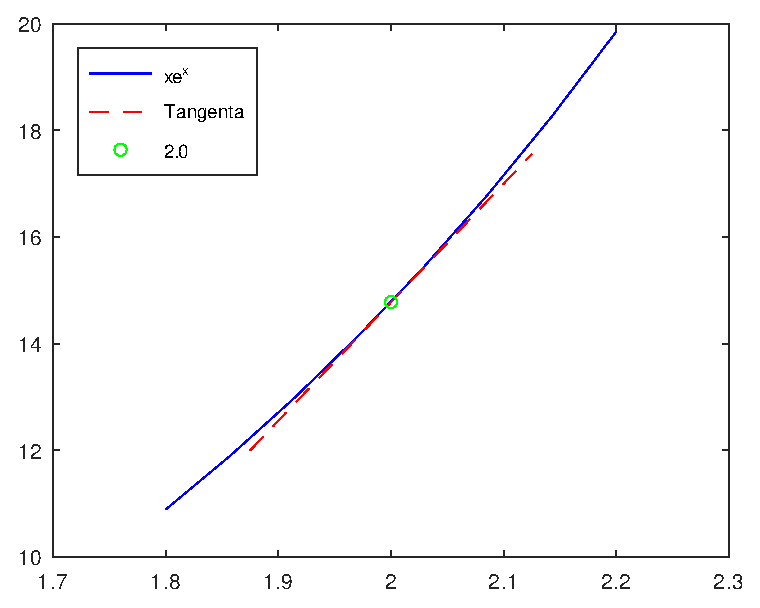
\includegraphics[scale=0.45]{three_points_mid_ex}
\end{minipage}
{\LARGE$\xrightarrow[]{Zoom}$}\;\;\;\;\;
\begin{minipage}{0.65\textwidth}
    \framebox{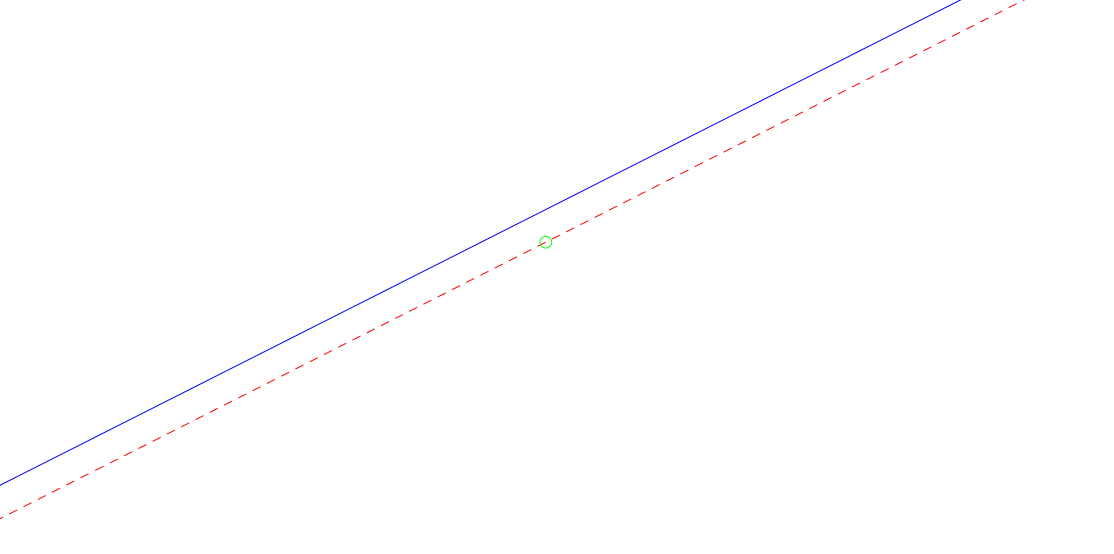
\includegraphics[scale=0.275]{three_points_mid_zoom}}
\end{minipage}\\

\subsubsection{Concluzii prima derivata}
\hspace{-1.25cm}\begin{minipage}{0.625\textwidth}
    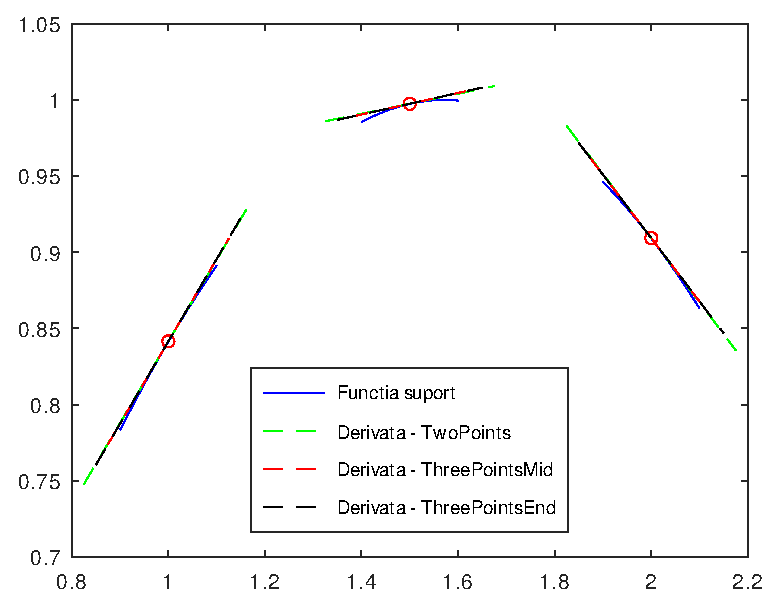
\includegraphics[scale=0.65]{comparatii_derivate}
\end{minipage}\hspace{-0.5cm}
\begin{minipage}{0.6\textwidth}
    \tabto{0.5cm} In figura alaturata se pot observa interpretarile grafice ale primei derivate obtinute prin cele $3$ formule determinate anterior: Two-Point(*), Three-Point-Endpoint(**), Three-Point-Midpoint(***)\\
    
    \tabto{0.5cm} Privind \textit{graficul}, pare ca cele $3$ metode conduc la aceeasi tangenta, insa daca analizam lucrurile din punct de vedere \textit{numeric}, observam ca metodele au diferite grade de acuratete. \\
    
    \vspace{0.25cm}\tabto{0.5cm} \textcolor{red}{Erorile de aproximatie:} $\begin{cases}
        (*): 7.95 \cdot 10^{-3} \\
        (**): 2.28 \cdot 10^{-5} \\
        (***): 1.14 \cdot 10^{-5} \\ 
    \end{cases}$ \\
    
    \tabto{0.5cm} Asadar, pentru functia suport, metoda (***) are cea mai buna acuratete. 
\end{minipage}\\


\subsection{A doua derivata}
\label{sec:sec_der}

\paragraph{Modul de determinare}

\tabto{0.5cm} In continuare, dorim sa aproximam $f''(x_0)$. Pornim de la dezvoltarea in serie Taylor\framebox[0.3cm][r]{\footnotemark} a functiei $f(x)$ in jurul punctului $x_0$:
\footnotetext{\framebox[8.25cm]{\url{https://en.wikipedia.org/wiki/Taylor_series\#Definition}}}
$f(x) = f(x_0) + (x-x_0)f'(x_0) + \frac{(x-x_0)^2}{2!}f''(x_0) + \frac{(x-x_0)^3}{3!}f^{(3)}(x_0) + \dots$\\

Pastram din seria Taylor, primii $3$ termeni:

$f(x) = f(x_0) + (x-x_0)f'(x_0) + \frac{(x-x_0)^2}{2!}f''(x_0) + \frac{(x-x_0)^3}{3!}f^{(3)}(x_0) + \textcolor{red}{\frac{(x-x_0)^4}{4!}f^{(4)}(\xi)}$\\

Facand, pe rand, \framebox{$x \rightarrow x_0+h$} si \framebox{$x \rightarrow x_0-h$}, obtinem:

\vspace{0.1cm}$\begin{cases}
    f(x_0+h) = f(x_0) + f'(x_0) h + \frac{1}{2} f''(x_0) h^2 + \frac{1}{6} f^{(3)}(x_0) h^3 + \textcolor{red}{\frac{1}{24} f^{(4)}(\xi_1) h^4} \vspace{0.1cm}\\
    f(x_0-h) = f(x_0) - f'(x_0) h + \frac{1}{2} f''(x_0) h^2 - \frac{1}{6} f^{(3)}(x_0) h^3 + \textcolor{red}{\frac{1}{24} f^{(4)}(\xi_{-1}) h^4}
\end{cases}$

Observatie: $x_0-h < \xi_{-1} < x_0 < \xi_1 < x_0+h$ \\

Insumam cele $2$ relatii membru cu membru si obtinem:

$f(x_0+h) + f(x_0-h) = 2f(x_0) + $\framebox{$f''(x_0)$}$ h^2 + \textcolor{red}{\frac{1}{24} [f^{(4)}(\xi_1) + f^{(4)}(\xi_{-1})] h^4}$

$\Longrightarrow$ 
\framebox{$f''(x_0) = \frac{1}{h^2} [f(x_0-h) - 2f(x_0) + f(x_0+h)] - \textcolor{red}{\frac{h^2}{24} [f^{(4)}(\xi_1) + f^{(4)}(\xi_{-1})]}$}\\

Presupunem ca $f^{(4)}$ este continua pe $[x_0-h, x_0+h]$.

Este evident ca $\frac{1}{2} [f^{(4)}(\xi_1) + f^{(4)}(\xi_{-1})]$ se afla intre $f^{(4)}(\xi_1)$ si $f^{(4)}(\xi_{-1})$.

Conform Toeremei de Medie\framebox[0.3cm][r]{\footnotemark}, exista o valoare $\xi$ intre $\xi_{-1}$ si $\xi_{1}$ si implicit in intervalul\;\;\; $[x_0-h, x_0+h]$, a.\^i.
$f^4(\xi) = \frac{1}{2} [f^{(4)}(\xi_1) + f^{(4)}(\xi_{-1})]$. Astfel, formula de aproximare a derivatei a II-a, se reduce la:
\footnotetext{\framebox[9.75cm]{\url{https://en.wikipedia.org/wiki/Intermediate_value_theorem\#Theorem}}}

\begin{mdframe16cm}
\vspace{-0.5cm}\paragraph{Second Derivative Midpoint Formula}
\tabto{0.5cm}\framebox{$f''(x_0) = \frac{1}{h^2} [f(x_0-h) - 2f(x_0) + f(x_0+h)] - \textcolor{red}{\frac{h^2}{12} f^{(4)}(\xi)}$}, cu $\xi \in (x_0-h, x_0+h)$ \textbf{(****)}
\end{mdframe16cm}

Astfel, am determinat formula cu care putem aproxima derivata a II-a a unei functii $f$. Privind puterea lui $h$, tragem concluzia ca aceasta este o metoda de \textbf{ordin 2}.

\paragraph{Exemplu numeric}

\begin{align*}
    \tabto{0.5cm}\begin{minipage}{0.4\textwidth}
    \tabto{0.5cm} Fie functia $f(x) = xe^x$. Aproximati $f''(2)$, cunoscand urmatorul suport de interpolare:
    \end{minipage}\hspace{1cm}
    \begin{minipage}{0.4\textwidth}
        \begin{tabular}{c | c}
            x & f(x) \\
            \hline
            1.8 & 10.889365 \\
            \hline
            1.9 & 12.703199 \\
            \hline
            \textbf{2.0} & \textbf{14.778112} \\
            \hline
            2.1 & 17.148957 \\
            \hline
            2.2 & 19.855030 \\
        \end{tabular}
    \end{minipage}
\end{align*}

Suportul de interpolare ne permite sa aproximam $f''(2)$ in $2$ moduri diferite:

Folosind \textbf{Second Derivative MidPoint (****)} cu pasul:
$\begin{cases}
    h = 0.1 \\
    $\;\;\;sau$ \\
    h = 0.2 \\
\end{cases}$ \\

\textit{Observatie:} Pentru limitele erorii de aproximare, tinem cont de faptul ca $f^{(4)}(x) = (x+3)e^x$\\

Folosind pasul $\mathbf{h=0.1}$, obtinem:
\tabto{1cm}$f''(2) = \frac{1}{(0.1)^2} [f(2-0.1) -2f(2) + f(2 + 0.1)]\Rightarrow$ \framebox{$f''(2) = 29.593200$} ($\xi \in (1.9, 2.1)$)
\tabto{1cm}$err(****)_{h=0.1} = \frac{|h^2 \cdot f^{(4)}(\xi)|}{12} = \frac{|h^2| \cdot (\xi+3)e^{\xi}}{12} < \frac{(0.1)^2 \cdot (2.1+3)e^{2.1}}{12} \Rightarrow$ \framebox{\textcolor{red}{$err(****)_{h=0.1} < 0.034$}}\\


Folosind pasul $\mathbf{h=0.2}$, obtinem:
\tabto{1cm}$f''(2) = \frac{1}{(0.2)^2} [f(2-0.2) -2f(2) + f(2 + 0.2)]\Rightarrow$ \framebox{$f''(2) = 29.704275$} ($\xi \in (1.8, 2.2)$)
\tabto{1cm}$err(****)_{h=0.2} = \frac{|h^2 \cdot f^{(4)}(\xi)|}{12} = \frac{|h^2| \cdot (\xi+3)e^{\xi}}{12} < \frac{(0.2)^2 \cdot (2.2+3)e^{2.2}}{12} \Rightarrow$ \framebox{\textcolor{red}{$err(****)_{h=0.2} < 0.156$}}\\

Derivata II a functiei $f(x) = xe^x$ este $f''(x) = (x+2)e^x$, deci valoarea \textit{exacta} a derivatei II a functiei $f(x)$ in punctul $2.0$ este $f''(2.0) = (2+2)e^2 =$ \framebox{$29.556224$}. Comparand cele $2$ aproximatii, observam ca cea mai apropiata de valoarea exacta este formula (****) cu pasul $h=0.1$


\subsection{Rezumat formule derivare}
% Cheatsheet
\begin{mdframe16cm}
    \vspace{0.25cm}\tabto{0.5cm}\textbf{Two-Point (*)}\\
    
    \tabto{1cm}\framebox{$f'(x_0) = \frac{f(x_0+h)-f(x_0)}{h} - \textcolor{red}{\frac{h}{2} \cdot f''(\xi)}$} ($\xi$ se afla intre $x_0$ si $x_0+h$)\\
    
    \tabto{0.5cm}\textbf{Three-Point-Endpoint (**)}\\
    
    \tabto{1cm}\framebox{$f'(x_0) = \frac{1}{2h}[-3f(x_0) + 4f(x_0+h) - f(x_0+2h)] + \textcolor{red}{\frac{h^2}{3}f^{(3)}(\xi)}$} ($\xi$ se afla intre $x_0$ si $x_0+2h$)\\
    
    \tabto{0.5cm}\textbf{Three-Point-Midpoint (***)}\\
    
    \tabto{1cm}\framebox{$f'(x_0) = \frac{1}{2h}[f(x_0+h) - f(x_0-h)] - \textcolor{red}{\frac{h^2}{6}f^{(3)}(\xi)}$} ($\xi$ se afla intre $x_0-h$ si $x_0+h$)\\
    
    \tabto{0.5cm}\textbf{Second Derivative Midpoint Formula (****)}
    \tabto{1cm}\framebox{$f''(x_0) = \frac{1}{h^2} [f(x_0-h) - 2f(x_0) + f(x_0+h)] - \textcolor{red}{\frac{h^2}{12} f^{(4)}(\xi)}$}, cu $\xi \in (x_0-h, x_0+h)$
\end{mdframe16cm}



\section{Integrare}


\subsection{Introducere}
\subsubsection{Notiuni generale}
\tab Fie o functie $f:[a,b]\rightarrow\mathbb{R}$. Dorim sa calculam, in mod aproximativ, integrala $\int_a^b f(x)\, dx$, cunoscand valorile functiei intr-un numar redus de puncte $(x_i, f(x_i)), \, i = \overline{0, n}$.


\subsubsection{Motivatie}
\tab Unele integrale sunt dificil de calculat folosind metode analitice. Astfel, introducem integrarea numerica prin \textbf{cuadraturi}.\framebox[0.3cm][r]{\footnotemark}
\footnotetext{\framebox[7.85cm]{\url{https://en.wikipedia.org/wiki/Numerical_integration}}}


\subsubsection{Idee}
\begin{minipage}{0.7\textwidth}
    \begin{itemize}
        \item Impartim intervalul $[a,b]$ in subintervale.
        \item Pe fiecare subinterval, aproximam functia $f(x)$ cu un polinom $P_i(x)$, obtinut prin \textit{interpolare}.
        \item Integram $P_i(x)$ pe fiecare subinterval si insumam rezultatele.
    \end{itemize}
\end{minipage}\hspace{0.75cm}
\begin{minipage}{0.5\textwidth}
    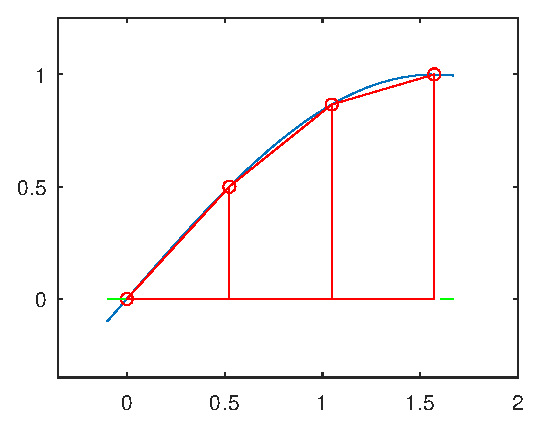
\includegraphics[scale=0.5]{ex_integrare_numerica}
\end{minipage}

\subsubsection{Moduri de aproximare abordate}
\begin{multicols}{2}
    \begin{itemize}
        \item \framebox{\textbf{\hyperref[sec:trapeze]{Regula trapezelor}}}
        \item \framebox{\textbf{\hyperref[sec:simpson]{Regula Simpson}}}
    \end{itemize}
    
    \begin{itemize}
        \item \framebox{\textbf{\hyperref[sec:adaptive]{Cuadraturi adaptive}}}
    \end{itemize}
\end{multicols}


\subsubsection{Aplicatii care folosesc integrarea numerica}

\tabto{0.5cm} Aplicatii precum calcularea de \textit{arii}, \textit{volume}, \textit{centrul de masa} sunt evidente pentru integrarea numerica. Vom prezenta, pe scurt, utilizarea integrarii numerica in studiul \textit{probabilitatilor}.

\paragraph{Studiul probabilitatilor}

\tabto{0.5cm} Dupa cum stiti, in studiul probabilitatilor, integralele definite sunt foarte intalnite.

De exemplu, pentru a determina \textit{functia de repartitie},\framebox[0.4cm][r]{\footnotemark}\hspace{-0.1cm}
\footnotetext{\framebox[9.5cm]{\url{https://en.wikipedia.org/wiki/Cumulative_distribution_function}}}
se poate calcula direct integrala definita.

Pentru mai multe detalii, puteti lectura materialul:
\href{https://www.whitman.edu/mathematics/calculus_online/section09.08.html}{
\includegraphics[scale=0.4]{document_button}}

\subsubsection{Pregatirea terenului}
\tab Inainte de a discutia despre fiecare mod de aproximare a integralei $\int_a^b f(x) \, dx$, prezentam cadrul discutiei:

\begin{itemize}
    \item Pornim de la o functie continua $f:[a,b]\rightarrow\mathbb{R}$ careia ii cunoastem valorile intr-un numar redus de puncte.
    \item Dorim sa gasim o aproximatie cat mai buna a integralei definite $\int_a^b f(x) \, dx$.
\end{itemize}

\tabto{0.5cm} Alegem $(n+1)$ puncte \textit{echidistante} (pentru metodele \textit{Newton-Cotes}) in intervalul $[a,b]$:

\framebox{$x_i = a_i + i \cdot h$},
$\begin{cases}
     i = 0 : n \\
     h = \frac{b-a}{n} \;$(lungimea subintervalului)$\\
\end{cases}$\\

Ideea de cuadratura numerica este data de aproximarea integralei definite printr-o \textit{suma}:

\framebox{$\int_a^b f(x) \, dx \simeq \sum\limits_{i=0}^{n} a_i f(x_i)$} \\

Ne propunem sa determinam coeficientii $a_i$. Aproximam functia $f(x)$ cu polinomul de interpolare Lagrange, metinand gradul $n$ cat mai mic: $f(x) \simeq P_n(x)$

$P_n(x) \; \eqdef \; \sum\limits_{i=0}^{n} f(x_i) L_i(x)$.

Asadar, facand aproximatia $f(x) \simeq P_n(x)$ si integrand in ambii membri, obtinem: 

$\int_a^b f(x) \, dx \simeq \int_a^b \sum\limits_{i=0}^{n} f(x_i) L_i(x) \, dx$
$\iff \int_a^b f(x) \, dx \simeq\sum\limits_{i=0}^{n} f(x_i) \cdot $\framebox{$\int_a^b L_i(x) \, dx$} \\

Dar, $\int_a^b f(x) \, dx \simeq \sum\limits_{i=0}^{n} f(x_i) \cdot $ $\framebox{$a_i$}$

$\xRightarrow[identificare]{Prin}$ \framebox{$a_i = \int_a^b L_i(x) \, dx$},$\; i = 0 : n$ \\

Asadar, pentru a aproxima $\int_a^b f(x) \, dx$, alegem coeficientii $a_i$ astfel: $a_i = \int_a^b L_i(x) \, dx$

Reamintim faptul ca $L_i(x)$ s.n. \textit{multiplicatori Lagrange} si se calculeaza astfel:
\framebox{$L_i(x) = \prod\limits_{\substack{j=0 \\ j\neq i}}^{n} \frac{x-x_j}{x_i-x_j},\; j = \overline{0, n}$}\\

In continuare, vom trata pe rand cazurile
$\begin{cases}
    n = 1 \;$(Trapez)$ \\
    n = 2 \;$(Simpson)$ \\
\end{cases}$


\subsection{Metode Newton-Cotes}
\subsubsection{Regula simpla a trapezelor (n=1)}
\label{sec:trapeze}

\paragraph{Modul de determinare}

\tabto{0.5cm} Dorim sa aproximam $\int_a^b f(x) \, dx$, folosind o interpolare polinomiala Lagrange de grad $n=1$ (interpolare liniara). Impartim intervalul $[a,b]$ intr-un subinterval $(n=1)$. \\

Atunci, abscisele vor fi: \framebox{$x_0 = a$} si \framebox{$x_1 = b$}, iar lungimea subintervalului: \framebox{$h = \frac{b-a}{1} = b-a$} \\

Asa cum am discutat, aproximam functia $f$ printr-un polinom de grad $n=1$: $f(x) \simeq P_1(x)$

$P_1(x) = f(x_0) \cdot \frac{x-x_1}{x_0-x_1} + f(x_1) \cdot \frac{x-x_0}{x_1-x_0}$

$\xRightarrow[]{|\int_a^b} \int_a^b f(x)\, dx \simeq \int_a^b P_1(x)\, dx$
$\iff \int_a^b f(x)\, dx \simeq \int_a^b [f(x_0) \cdot \frac{x-x_1}{x_0-x_1} + f(x_1) \cdot \frac{x-x_0}{x_1-x_0}]\, dx~\eqdots~\frac{h}{2} [f(a)~+~f(b)]$ \\


Astfel, am determinat formula pentru \textit{Regula Simpla a Trapezelor}:

\begin{mdframe16cm}
    \vspace{-0.5cm}\paragraph{Regula Simpla a Trapezelor}
    \tabto{0.5cm}\framebox{$\int_a^b f(x)\, dx \simeq \frac{h}{2} [f(a) + f(b)]$} \textbf{(*)} (reamintim faptul ca $h=b-a$)
\end{mdframe16cm}

\paragraph{Interpretarea geometrica}

\tabto{0.5cm} Cand functia $f$ ia valori pozitive pe $[a,b]$, integrala $\int_a^b f(x)\, dx$ este aproximata cu \textit{aria unui trapez}. De aici si denumirea de \textit{Regula Trapezelor}. \\

Formula (*) poate fi determinata si geometric - Aproximam integrala cu aria trapezului:

$\int_a^b f(x)\, dx \simeq \frac{[Baza_{mare} + Baza_{mica}] \cdot Inaltimea}{2} \iff \int_a^b f(x)\, dx \simeq \frac{[f(x_1) + f(x_0)] \cdot [x_1 - x_0]}{2}$\\

\paragraph{Exemplu numeric}

\tabto{0.5cm}\begin{minipage}{0.7\textwidth}
    \vspace{0.5cm}\tabto{0.5cm} Fie functia $f(x) = e^x$, $x \in [0, 2]$. Aproximati $\int_0^2 f(x)\, dx$, folosind \textit{Regula Simpla a Trapezelor}. \\
    
    \tabto{0.5cm} Pur si simplu, aplicam formula (*):
    $\int_0^2 f(x)\, dx \simeq \frac{h}{2} \cdot [f(0) + f(2)]$,
    
    \hspace{0.5cm}unde $h = b-a = 2-0 = 2$. 
    
    \tabto{0.5cm} Deci, $\int_0^2 f(x)\, dx \simeq \frac{2}{2} \cdot [e^0 + e^2] \Longrightarrow$ \framebox{$\int_0^2 f(x)\, dx \simeq 8.389$} \\
    
    \tabto{0.5cm} \textit{Observatie:} Valoarea exacta a integralei este $\int_0^2 f(x)\, dx = 6.389$
    
    \tabto{0.5cm} Asadar, aproximatia cu trapez simplu nu este cea mai buna.
\end{minipage}\hspace{0.5cm}
\begin{minipage}{0.5\textwidth}
    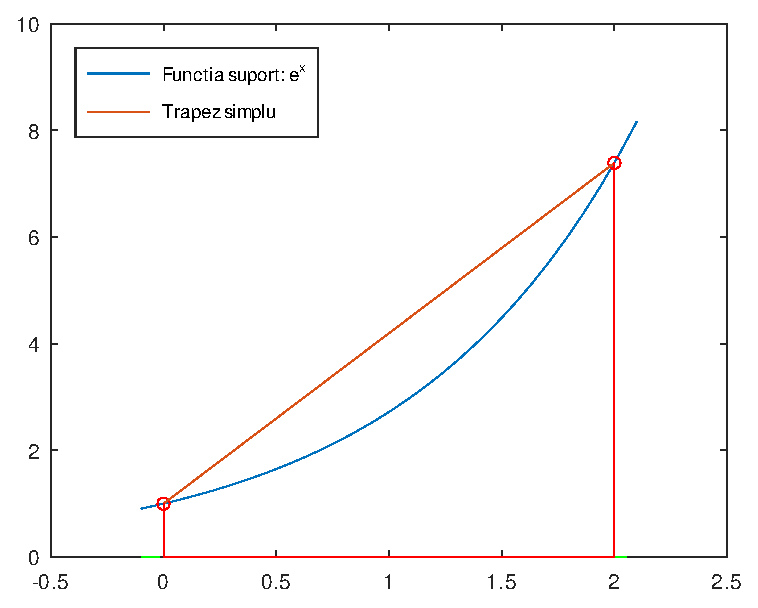
\includegraphics[scale=0.4]{trapez_simplu_ex}
\end{minipage}\\

\paragraph{Ce putem imbunatati?}
\tabto{0.5cm} In loc sa integram pe tot intervalul, putem sa impartim problema in probleme mai mici, aplicand regula simpla a trapezelor pe subintervale.


\subsubsection{Regula compusa a trapezelor}
\paragraph{Modul de determinare}

\tabto{0.5cm}\begin{minipage}{0.7\textwidth}
    \tabto{0.5cm} Regula simpla a trapezelor discutata anterior, este utila atunci cand intergram o singura data, pe tot intervalul $[a,b]$.
    
    \tabto{0.5cm} Pentru a ne apropia de o aproximatie mai buna a integralei $\int_a^b f(x)\, dx$, trebuie sa divizam problema in sub-probleme:
    
    \tabto{0.5cm} Impartim intervalul $[a,b]$ in $n$ subintervale de \textit{lungimi egale}: 
    
    $x_i = a + i \cdot h$, $i = 0:n$ si $h=\frac{b-a}{n}$
\end{minipage}
\begin{minipage}{0.7\textwidth}
    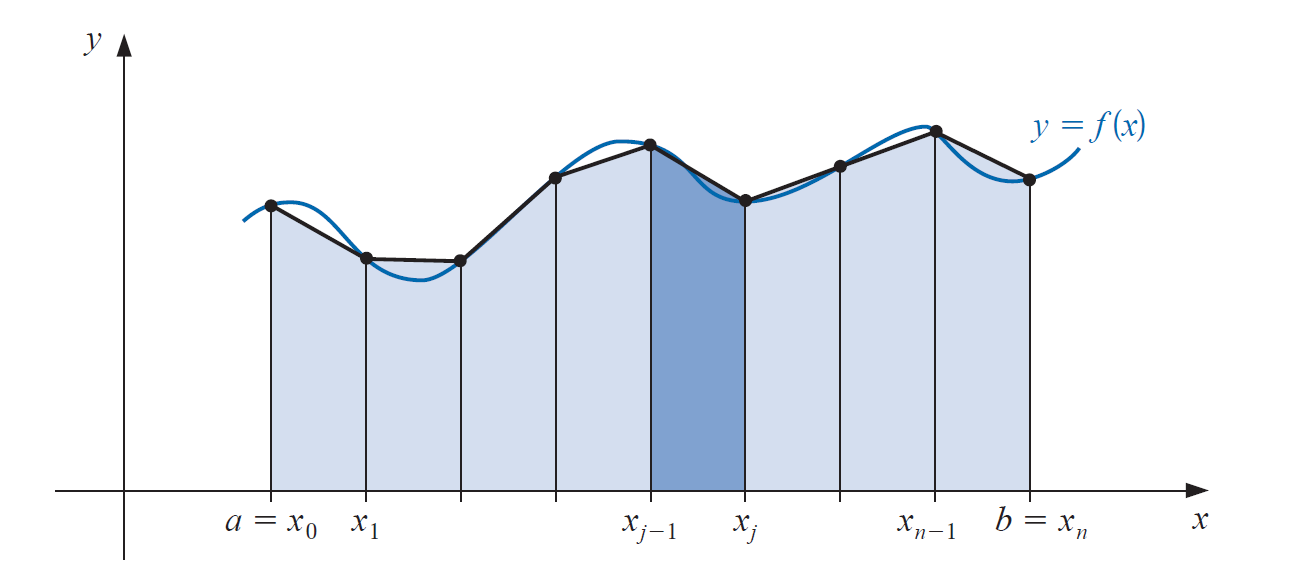
\includegraphics[scale=0.25]{trapez_compus_grafic}
\end{minipage}\vspace{0.25cm}

Atunci, $\int_a^b f(x)\, dx = \int_{x_0}^{x_n} f(x)\, dx =  \int_{x_0}^{x_1} f(x)\, dx +  \int_{x_1}^{x_2} f(x)\, dx + \dots +  \int_{x_n-1}^{x_n} f(x)\, dx$ \vspace{0.1cm}

Apoi, aplicam regula simpla a trapezelor pe fiecare subinterval. 

Astfel, integrala se poate aproxima:
$\int_a^b f(x)\, dx \simeq \sum\limits_{i=0}^{n-1} \frac{h}{2} \cdot [f(x_i) + f(x_{i+1})]$

$\Rightarrow \int_a^b f(x)\, dx \simeq \frac{h}{2} \cdot [f(x_0) + f(x_1) + f(x_1) + f(x_2) + \dots + f(x_{n-1}) + f(x_n)]$

$\Rightarrow \int_a^b f(x)\, dx \simeq \frac{h}{2} \cdot [f(x_0) + f(x_n) + 2 \sum\limits_{i=1}^{n-1} f(x_i)]$ \\

Astfel, am determinat formula pentru \textit{Regula Compusa a Trapezelor}:

\begin{mdframe16cm}
    \vspace{-0.5cm}\paragraph{Regula Compusa a Trapezelor}
    \tabto{0.5cm}\framebox{$\int_a^b f(x)\, dx \simeq h \cdot [\frac{f(x_0) + f(x_n)}{2} + \sum\limits_{i=1}^{n-1} f(x_i)] \; \eqnot \; T(f;h)$}, $h = \frac{b-a}{n}\;$ \textbf{(**)}
\end{mdframe16cm}

\tabto{0.5cm} \textit{Avantajul} gruparii termenilor in aceasta forma este ca se poate \textbf{vectoriza}.\framebox[0.4cm][r]{\footnotemark}
\footnotetext{\framebox[10cm]{\url{https://stackoverflow.com/questions/1422149/what-is-vectorization}}}


\paragraph{Analiza erorii}

\tabto{0.5cm}Facem urmatoarele notatii:
$\begin{cases}
    T(f;h) \equiv \; $aproximatia integralei folosind regula compusa a trapezelor$ \\
    I(f) \equiv \; $valoarea exacta a integralei$ \\
    \textcolor{red}{E_T(f;h)} \equiv \; $eroarea trapezoidala pentru functia $f$ cu pas $ h \\
\end{cases}$\\

Eroarea totala se poate scrie astfel: $\textcolor{red}{E_T(f;h)} = I(f) - T(f;h) = \sum\limits_{i=0}^{n-1} \int_{x_i}^{x_{i+1}} [f(x) - P_1(x)]\, dx$

$\Rightarrow \textcolor{red}{E_T(f;h)} = \sum\limits_{i=0}^{n-1} E_{T,i}(f;h)$, unde cu $E_{T,i}(f;h)$ am notat eroarea pe subintervalul $[x_i, x_{i+1}]$.

Practic, este eroarea provenita in urma interpolarii polinomiale pe subintervalul $i$. \\

Confrom \textit{\hyperref[sec:est_err]{teoremei de estimare a erorii}}:

$\textcolor{red}{E_{T,i}(f;h)} = \int_{x_i}^{x_{i+1}} \frac{1}{2} f''(\xi_i) (x-x_i) (x-x_{i+1})\, dx = \frac{1}{2} f''(\xi_i) \cdot \int_{x_i}^{x_{i+1}} (x-x_i) (x-x_{i+1})\, dx$

$\xRightarrow[]{(...)} \textcolor{red}{E_{T,i}(f;h)} = -\frac{1}{12} h^3 \cdot f''(\xi_i),\; \xi_i \in (x_i, x_{i+1})$ \\

Insumam erorile \textit{locale} si obtinem eroarea \textit{globala}:
$\textcolor{red}{E_T(f;h)} = \sum\limits_{i=0}^{n-1} E_{T,i}(f;h) = \sum\limits_{i=0}^{n-1} -\frac{h^3}{12} \cdot f''(\xi_i)$

Completam cu $\frac{1}{n}$:
$\textcolor{red}{E_T(f;h)} = -\frac{h^3}{12} \cdot [\sum\limits_{i=0}^{n-1} f''(\xi_i)] \cdot \frac{1}{n} \cdot n$

Tinem cont ca $f''$ continua, deci exista o medie a valorilor:
$\textcolor{red}{E_T(f;h)} = -\frac{h^3}{12} \cdot f''(\xi) \cdot n,\; \xi \in (a,b)$\vspace{0.2cm}

Reamintim ca $n = \frac{b-a}{h}$:
$\textcolor{red}{E_T(f;h)} = -\frac{b-a}{12} \cdot h^2 \cdot f''(\xi), \; \xi \in (a,b)$

$\xRightarrow[]{|\,|}$ \framebox{$|\textcolor{red}{E_T(f;h)}| \leq \frac{b-a}{12} \cdot h^2 \cdot \max\limits_{x \in (a,b)}^{} |f''(x)|$} \\

Astfel, am determinat limitele erorii totale pentru \textit{Regula Compusa a Trapezelor}.

Exponentul lui $h$ ne indica faptul ca formula este o metoda de \textbf{ordin 2}.


\paragraph{Exemplu numeric}

\tabto{0.5cm}\begin{minipage}{0.8\textwidth}
    \vspace{0.5cm}\tabto{0.5cm} Fie functia $f(x) = e^x$, $x \in [0, 2]$. Aproximati $\int_0^2 f(x)\, dx$ cu \textit{Regula Compusa a Trapezelor}, folosind $n=4$ subintervale. \\
    
    \tabto{0.5cm} Pur si simplu, aplicam formula (**), pentru $n=4$:
    
    $\int_0^2 f(x)\, dx \simeq h \cdot [\frac{f(0) + f(2)}{2} + f(0.5) + f(1) + f(1.5)]$, unde $h = \frac{b-a}{n} = \frac{2-0}{4} = 0.5$. \\
    
    \tabto{0.5cm} Deci, $\int_0^2 f(x)\, dx \simeq 0.5 \cdot [\frac{e^0 + e^2}{2} + e^{0.5} + e^1 + e^{1.5}] \Longrightarrow$ \framebox{$\int_0^2 f(x)\, dx \simeq 6.521$} \\
    
    \tabto{0.5cm} \textit{Observatie:} Valoarea exacta a integralei este $\int_0^2 f(x)\, dx = 6.389$
    
    \tabto{0.5cm} Asadar, am obtinut o aproximatie mult mai buna fata de trapez simplu.
\end{minipage}\hspace{0.1cm}
\begin{minipage}{0.55\textwidth}
    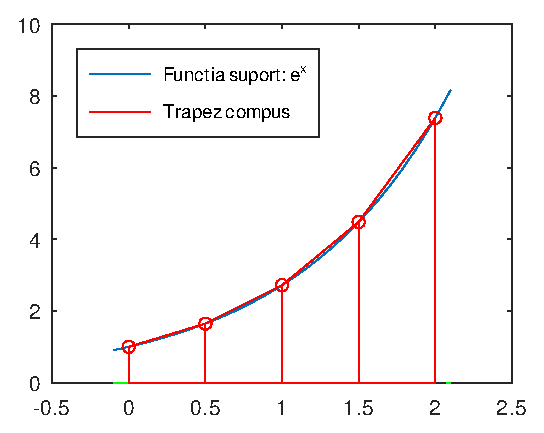
\includegraphics[scale=0.6]{trapez_compus_ex}
\end{minipage}\\

\tabto{0.5cm} Pentru a intelege mai bine cum lucreaza \textit{Regula Compusa a Trapezelor}, puteti urmari aceasta~\framebox{\href{https://imgur.com/a/bCqdgOG}{Animatie}}

\tabto{0.5cm} \textit{Cerinta suplimentara:} Care este numarul minim de subintervale prin care putem aproxima integrala $\int_0^2 e^x\, dx$, folosind \textit{Regula Compusa a Trapezelor}, cu o \textcolor{red}{eroare} mai mica de $\textcolor{blue}{0.5 \cdot 10^{-4}}$? \\

Ne folosim de inegalitatea:
$|\textcolor{red}{E_T(f;h)}| \leq \frac{b-a}{12} \cdot h^2 \cdot \max\limits_{x \in (a,b)}^{} |f''(x)|\;$
si tinem cont ca 
$\begin{cases}
    f''(x) = e^x,\, f'' $ continua$ \\
    a = 0 \\
    b = 2 \\
\end{cases}$

Inlocuim $\max\limits_{x \in (0,2)}^{} |f''(x)| = e^2$ in inegalitatea de mai sus si obtinem:

$|\textcolor{red}{E_T(f;h)}| \leq \frac{2-0}{12} \cdot h^2 \cdot e^2 \leq \textcolor{blue}{0.5 \cdot 10^{-4}} \iff h^2 \leq 0.5 \cdot 10^{-4} \cdot 6 \cdot e^{-2} \simeq 4.06 \cdot 10^{-5}$

Dar, $h = \frac{2-0}{n}$. Atunci, inegalitatea devine:
$\frac{2-0}{n} \leq \sqrt{4.06 \cdot 10^{-5}} \Rightarrow$ \framebox{$n \geq 314$} \\

Asadar, avem nevoie de cel putin $314$ subintervale ($315$ puncte) pentru a aproxima integrala cu o \textcolor{red}{eroare} mai mica de $\textcolor{blue}{0.5 \cdot 10^{-4}}$. In concluzie, \textit{foarte multe puncte}.

\paragraph{Ce putem imbunatati?}
\tabto{0.5cm} Putem creste gradul polinomului de interpolare Lagrange de la $n=1$ la $n=2$. Astfel, introducem in discutie \textit{Regula Simpson}.


\subsubsection{Regula simpla Simpson (n=2)}
\label{sec:simpson}

\paragraph{Modul de determinare}
\tabto{0.5cm} De data aceasta, suportul interpolarii este format din $n+1=2+1=3$ puncte ($x_0, x_1, x_2$).
\tabto{0.5cm} Asadar, mai avem un punct $x_1$ in mijlocul intervalului $[x_0, x_2]$ $\Rightarrow$ Aproximatie mai buna a functiei, implicit a integralei. \\

Putem determina \textit{Formula Simpla Simpson} in $2$ moduri:
\begin{itemize}
    \item Interpolam Lagrange (Analog trapezelor)
    \item Pornim de la dezvoltarea in serie Taylor a functiei $f$ in punctul $x_1$, pastrand primii $3$ termeni si folosind aproximatia derivatei a II-a, invatate anterior.
\end{itemize}

In cele ce urmeaza, vom exemplifica varianta cu interpolare Lagrange: \\


Impartim intervalul $[a,b]$ in $n=2$ subintervale.

Atunci, abscisele vor fi: \framebox{$x_0 = a$} si \framebox{$x_1 = \frac{a+b}{2}$}, \framebox{$x_2=b$}, iar lungimea subintervalului: \framebox{$h = \frac{b-a}{2}$} \\

Polinomul de interpolare Lagrange de grad $n=2$:

$P_2(x) = \frac{(x-x_1)(x-x_2)}{(x_0-x_1)(x_0-x_2)}f(x_0) + \frac{(x-x_0)(x-x_2)}{(x_1-x_0)(x_1-x_2)}f(x_1) + \frac{(x-x_0)(x-x_1)}{(x_2-x_0)(x_2-x_1)}f(x_2)$ \\

Asadar, pornim de la aproximatia $f(x) \simeq P_2(x)$ si intergram in ambii membri:

$\int_a^b f(x)\, dx \simeq \int_{x_0}^{x_2} [\frac{(x-x_1)(x-x_2)}{(x_0-x_1)(x_0-x_2)}f(x_0) + \frac{(x-x_0)(x-x_2)}{(x_1-x_0)(x_1-x_2)}f(x_1) + \frac{(x-x_0)(x-x_1)}{(x_2-x_0)(x_2-x_1)}f(x_2)]\, dx$ \newpage

$\int_a^b f(x)\, dx \simeq 
\frac{f(x_0)}{2h^2} \cdot \int_{x_0}^{x_2} (x-x_1)(x-x_2)\, dx$

\hspace{1.75cm}$- \frac{f(x_1)}{h^2} \cdot \int_{x_0}^{x_2} (x-x_0)(x-x_2)\, dx$ 

\hspace{1.75cm}$+ \frac{f(x_2)}{2h^2} \cdot \int_{x_0}^{x_2} (x-x_0)(x-x_1)\, dx$ \\

\hspace{-0.5cm}$\Rightarrow$
$\int_a^b f(x)\, dx \simeq$
$\frac{f(x_0)}{2h^2} \cdot \frac{2h^3}{3}$
$- \frac{f(x_1)}{h^2} \cdot \frac{-4h^3}{3}$
$+ \frac{f(x_2)}{2h^2} \cdot \frac{2h^3}{3}$
$\iff$
$\int_a^b f(x)\, dx \simeq$
$f(x_0) \cdot \frac{h}{3} + f(x_1) \cdot \frac{4h}{3} + f(x_2) \cdot \frac{h}{3}$ \\

Astfel, am determinat formula pentru \textit{Regula Simpla Simpson}:
\begin{mdframe16cm}
    \vspace{-0.5cm}\paragraph{Regula Simpla Simpson}
    \tabto{0.5cm}\framebox{$\int_a^b f(x)\, dx \simeq \frac{h}{3} \cdot [f(a) + 4f(\frac{a+b}{2}) + f(b)]$}, $h = \frac{b-a}{2}\;$ \textbf{(***)}
\end{mdframe16cm}


\paragraph{Exemplu numeric}

\tabto{0.5cm}\begin{minipage}{0.7\textwidth}
    \vspace{0.5cm}\tabto{0.5cm} Fie functia $f(x) = e^x$, $x \in [0, 2]$. Aproximati $\int_0^2 f(x)\, dx$, folosind \textit{Regula Simpla Simpson}. \\
    
    \tabto{0.5cm} Pur si simplu, aplicam formula (***):
    
    \hspace{0.45cm}$\int_0^2 f(x)\, dx \simeq \frac{h}{3} \cdot [f(0) + 4f(\frac{0+2}{2}) + f(2)]$, unde $h = \frac{b-a}{2} = \frac{2-0}{2} = 1$. \\
    
    \tabto{0.5cm} Deci, $\int_0^2 f(x)\, dx \simeq \frac{1}{3} \cdot [e^0 + 4 \cdot e^1 + e^2] \Longrightarrow$ \framebox{$\int_0^2 f(x)\, dx \simeq 6.420$} \\
    
    \tabto{0.5cm} \textit{Observatie:} Valoarea exacta a integralei este $\int_0^2 f(x)\, dx = 6.389$
    
    \tabto{0.5cm} Asadar, metodele incep sa se apropie de valoarea exacta.
\end{minipage}\hspace{0.5cm}
\begin{minipage}{0.5\textwidth}
    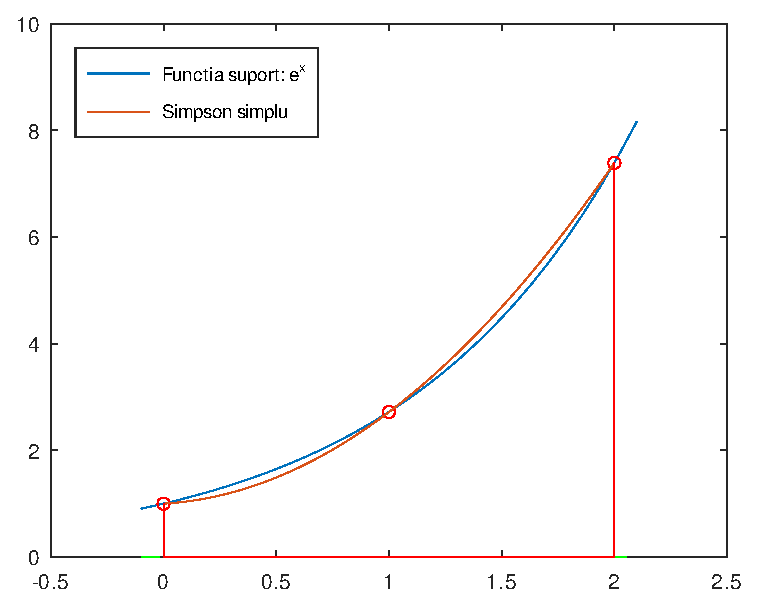
\includegraphics[scale=0.4]{simpson_simplu_ex}
\end{minipage}\\

\paragraph{Ce putem imbunatati?}
\tabto{0.5cm} La fel ca la trapeze, in loc sa integram pe tot intervalul, impartim problema in probleme mai mici, aplicand regula simpla Simpson pe subintervale.


\subsubsection{Regula compusa Simpson}

\paragraph{Modul de determinare}

\tabto{0.5cm}\begin{minipage}{0.7\textwidth}
    \tabto{0.5cm} Regula simpla Simpson discutata anterior, este utila atunci cand intergram o singura data, pe tot intervalul $[a,b]$.
    
    \tabto{0.5cm} Pentru a ne apropia de o aproximatie si mai buna a integralei $\int_a^b f(x)\, dx$, trebuie sa divizam problema in sub-probleme:
    
    \tabto{0.5cm} Impartim intervalul $[a,b]$ in $(2n)$ subintervale de \textit{lungimi egale}: $x_i = a + i \cdot h$, $i = 0:2n$ si $h=\frac{b-a}{2n}$
\end{minipage}
\begin{minipage}{0.7\textwidth}
    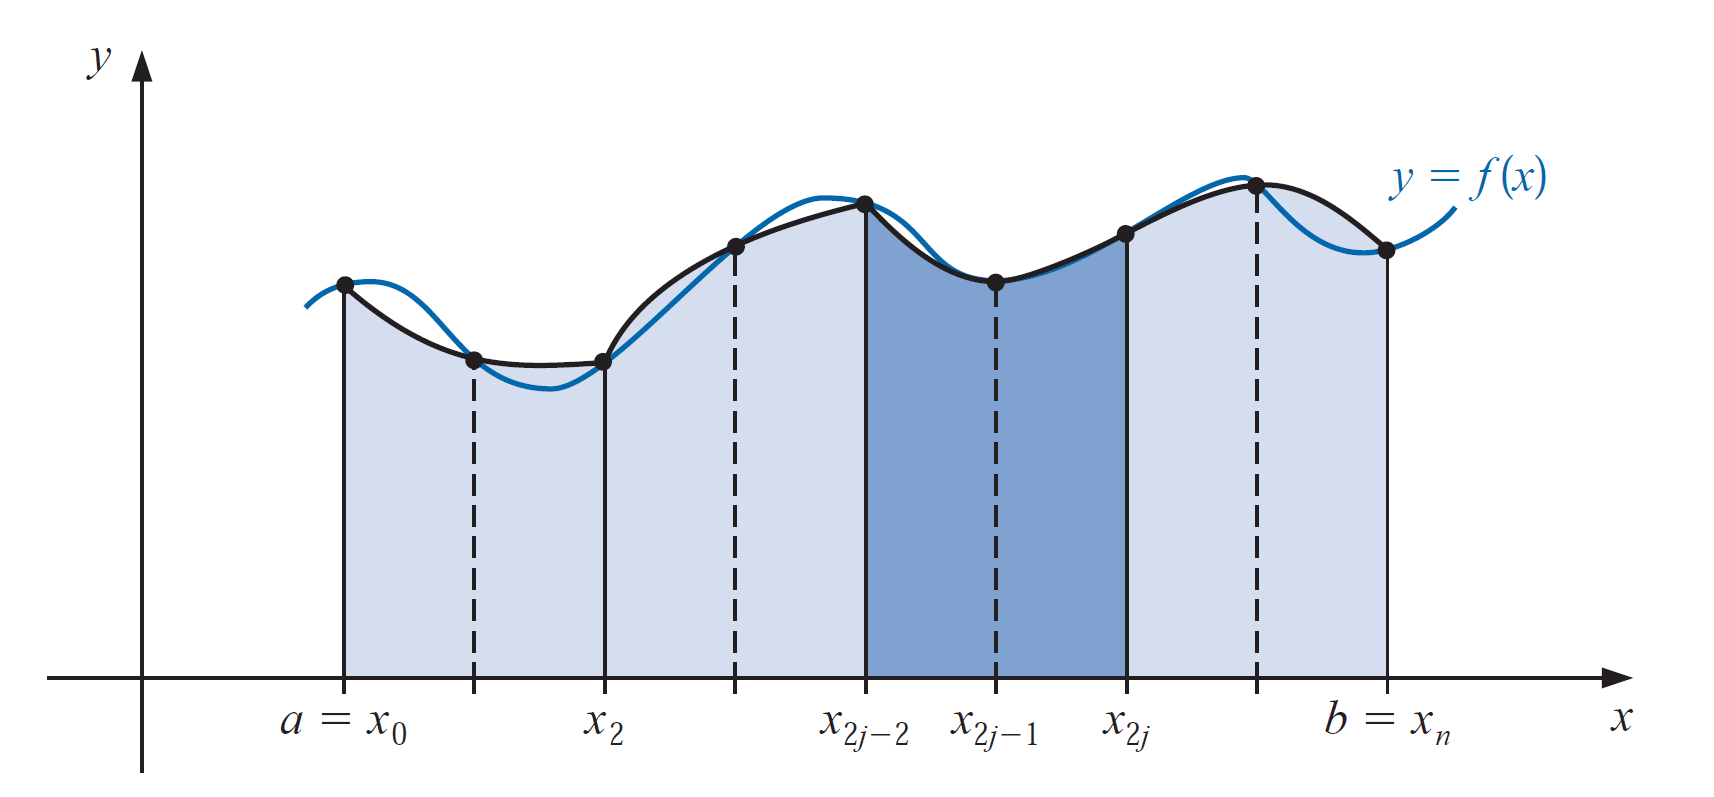
\includegraphics[scale=0.185]{simpson_compus_grafic}
\end{minipage}\vspace{0.25cm}

Apoi, aplicam regula simpla Simpson pe fiecare subinterval. 

Astfel, integrala se poate aproxima:
$\int_a^b f(x)\, dx \simeq \sum\limits_{i=1}^{n} \frac{h}{3} \cdot [f(x_{2i-2}) + 4f(x_{2i-1}) + f(x_{2i})]$

$\Rightarrow \int_a^b f(x)\, dx \simeq \frac{h}{3} [f(x_0) + 2 \cdot \sum\limits_{i=1}^{n-1} f(x_{2i}) + 4 \cdot \sum\limits_{i=1}^{n} f(x_{2i-1}) + f(x_{2n})] $

Astfel, am determinat formula pentru \textit{Regula Compusa Simpson}:

\begin{mdframe16cm}
    \vspace{-0.5cm}\paragraph{Regula Compusa Simpson}
    \tabto{0.5cm}\framebox{$\int_a^b f(x)\, dx \simeq \frac{h}{3} \cdot [f(x_0) + f(x_{2n}) + 4 \cdot \sum\limits_{i=1}^{n} f(x_{2i-1}) + 2 \cdot \sum\limits_{i=1}^{n-1} f(x_{2i})] \; \eqnot \; S(f;h)$}, $h = \frac{b-a}{2n}\;$ \textbf{(****)}
\end{mdframe16cm}

\tabto{0.5cm} La fel ca la trapeze, \textit{avantajul} gruparii termenilor in aceasta forma este ca se poate \textbf{vectoriza}. \newpage


\paragraph{Analiza erorii}

\tabto{0.5cm}Facem urmatoarele notatii:
$\begin{cases}
    S(f;h) \equiv \; $aproximatia integralei folosind regula compusa Simpson$ \\
    I(f) \equiv \; $valoarea exacta a integralei$ \\
    \textcolor{red}{E_S(f;h)} \equiv \; $eroarea Simpson pentru functia $f$ cu pas $ h \\
    \textcolor{red}{E_{S,i}(f;h)} \equiv \; $eroarea Simpson pe subintervalul $i$ $ \\
\end{cases}$ \\

Se procedeaza in mod analog \textit{erorii trapezelor} si se gaseste ca eroarea pe subintervalul $i$ este:

$\textcolor{red}{E_{S,i}(f;h)} = -\frac{h^5}{90} \cdot f^{(4)}(\xi_i),\; \xi_i \in (x_{2i}, x_{2i+2})$ \\

Insumam erorile \textit{locale} si obtinem eroarea \textit{totala}:
$\textcolor{red}{E_S(f;h)} = I(f) - S(f;h)$

$\Rightarrow \textcolor{red}{E_S(f;h)} = -\frac{1}{90} \cdot h^5 \cdot [\sum\limits_{i=0}^{n-1} f^{(4)}(\xi_i)] \cdot \frac{1}{n} \cdot n\;$ (am completat cu $n$)

Tinem cont ca $f^{(4)}$ continua, deci exista o medie a valorilor:

$\Rightarrow \textcolor{red}{E_S(f;h)} = -\frac{h^5}{90} \cdot f^{(4)}(\xi) \cdot \frac{b-a}{2h},\, \xi \in (a, b)\;$ (reamintim ca $n=\frac{b-a}{2h}$) \\

$\xRightarrow[]{|\,|}$ \framebox{$|\textcolor{red}{E_S(f;h)}| \leq \frac{b-a}{180} \cdot h^4 \cdot \max\limits_{x \in (a,b)}^{} |f^{(4)}(x)|$} \\

Astfel, am determinat limitele erorii totale pentru \textit{Regula Compusa Simpson}.

Exponentul lui $h$ ne indica faptul ca formula este o metoda de \textbf{ordin 4}.


\paragraph{Exemplu numeric}

\tabto{0.5cm}\begin{minipage}{0.8\textwidth}
    \vspace{0.5cm}\tabto{0.5cm} Fie functia $f(x) = e^x$, $x \in [0, 2]$. Aproximati $\int_0^2 f(x)\, dx$ cu \textit{Regula Compusa Simpson}, folosind $n=4$ subintervale. 
    
    \tabto{0.5cm} Pur si simplu, aplicam formula (****), pentru $n=4$:
    
    $\int_0^2 f(x)\, dx \simeq \frac{h}{3} \cdot \{f(x_0) + f(x_{8}) + 4 \cdot [f(x_1) + f(x_3) + f(x_5) + f(x_7)] + 2 \cdot  [f(x_2) + f(x_4) + f(x_6)]\}$, unde $h = \frac{b-a}{2n} = \frac{2-0}{8} = 0.25$. \\
    
    \tabto{0.5cm} Deci, $\int_0^2 f(x)\, dx \simeq \frac{0.25}{3} \cdot [e^0 + e^2 + 4 \cdot (e^{0.25} + e^{0.75} + e^{1.25} + e^{1.75}) + 2 \cdot (e^{0.5} + e^1 + e^{1.5})] \Longrightarrow$ \framebox{$\int_0^2 f(x)\, dx \simeq 6.38919$} \\
    
    \tabto{0.5cm} \textit{Observatie:} Valoarea exacta a integralei este $\int_0^2 f(x)\, dx = 6.38906$
    
    \tabto{0.5cm} Asadar, am obtinut o aproximatie foarte buna, considerand doar $n=4$.
\end{minipage}\hspace{0.1cm}
\begin{minipage}{0.55\textwidth}
    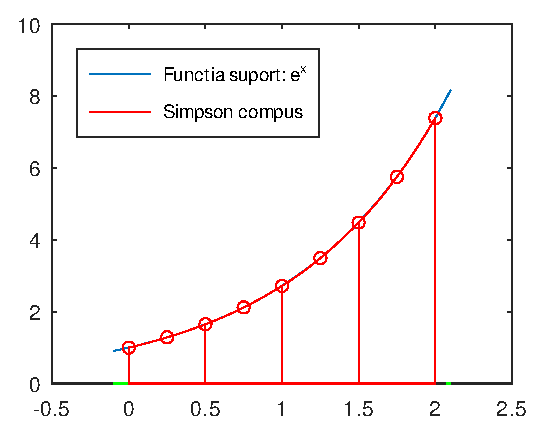
\includegraphics[scale=0.6]{simpson_compus_ex}
\end{minipage}\\

\tabto{0.5cm} Pentru a intelege mai bine cum lucreaza \textit{Regula Compusa Simpson}, puteti urmari aceasta~\framebox{\href{https://imgur.com/a/uAxm67c}{Animatie}}


\tabto{0.5cm} \textit{Cerinta suplimentara:} Care este numarul minim de subintervale prin care putem aproxima integrala $\int_0^2 e^x\, dx$, folosind \textit{Regula Compusa Simpson}, cu o \textcolor{red}{eroare} mai mica de $\textcolor{blue}{0.5 \cdot 10^{-4}}$? \\

Ne folosim de inegalitatea:
$|\textcolor{red}{E_S(f;h)}| \leq \frac{b-a}{180} \cdot h^4 \cdot \max\limits_{x \in (a,b)}^{} |f^{(4)}(x)|\;$
si tinem cont ca 
$\begin{cases}
    f^{(4)}(x) = e^x,\, f^{(4)} $ continua$ \\
    a = 0 \\
    b = 2 \\
\end{cases}$

Inlocuim $\max\limits_{x \in (0,2)}^{} |f^{(4)}(x)| = e^2$ in inegalitatea de mai sus si obtinem:

$|\textcolor{red}{E_S(f;h)}| \leq \frac{2-0}{180} \cdot h^4 \cdot e^2 \leq \textcolor{blue}{0.5 \cdot 10^{-4}} \iff h^4 \leq 0.5 \cdot 10^{-4} \cdot \frac{180}{2e^2} \simeq 6.09 \cdot 10^{-4}$

Dar, $h = \frac{2-0}{2n}$. Atunci, inegalitatea devine:
$\frac{2-0}{2n} \leq \sqrt[4]{6.09 \cdot 10^{-4}} \Rightarrow$ \framebox{$n \geq 7$} \\

Asadar, avem nevoie de cel putin $7$ subintervale ($2 \cdot 7 + 1 = 15$ puncte) pentru a aproxima integrala cu o \textcolor{red}{eroare} mai mica de $\textcolor{blue}{0.5 \cdot 10^{-4}}$.

Daca va aduceti aminte, la \textit{Trapez Compus} (ordin 2) era nevoie de $315$  puncte, pe cand la \textit{Simpson Compus} (ordin 4) sunt necesare doar $15$ puncte, pentru aceeasi aproximatie (si aceeasi complexitate).


\paragraph{Ce putem imbunatati?}
\tabto{0.5cm} Pana acum, am lucrat cu metode care implica divizarea intervalului $[a,b]$ in subintervale de \textit{lungimi egale}.

In continuare, ne vom ocupa de o tehnica de aproximare a integralelor care nu necesita puncte echidistante.


\subsection{Cuadraturi adaptive}
\label{sec:adaptive}


\subsubsection{Notiuni generale}
\tab \textit{Eroarea locala} pentru aproximarea unei integrale este mare acolo unde functia se schimba mult (derivatele $f^{(k)}$ sunt mari).

Folosind subintervale egale (ca pana acum), irosim efort in zonele in care functia nu se schimba foarte mult. Regulile compuse discutate anterior sunt foarte utile, insa au de suferit pentru ca necesita puncte echidistante.


\subsubsection{Motivatie}

\vspace{0.5cm}\begin{minipage}{0.8\textwidth}
    \tabto{0.5cm} Sa consideram urmatoarea ecuatie diferentiala:
    $y'' + 6y' + 25 = 0$, avand urmatoarele conditii initiale
    $\begin{cases}
        y(0) = 0 \\
        y'(0) = 4 \\
    \end{cases}$ \\
    
    \tabto{0.5cm} Rezolvand analitic ecuatia diferentiala, obtinem solutia unica 
    
    $y(x) = e^{-3x} \cdot sin(4x)$ 
    
    \tabto{0.5cm} Functii de acest tip sunt foarte intalnite in \textit{ingineria mecanica} (descriu anumite caracteristici ale resorturilor, amortizoarelor) si in \textit{ingineria electrica} (sunt solutii pentru circuite electrice).
    
    \tabto{0.5cm} Graficul functiei $y(x) = e^{-3x} \cdot sin(4x)$  este ilustrat in figura alaturata.
\end{minipage}
\begin{minipage}{0.25\textwidth}
    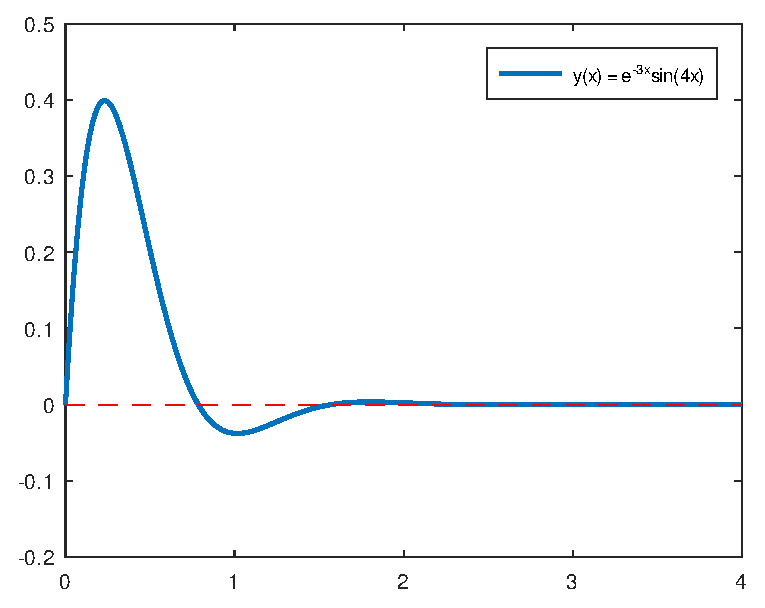
\includegraphics[scale=0.45]{fct_cuad_ad}
\end{minipage} \\

\tabto{0.5cm} Sa presupunem ca vrem sa calculam integrala $\int_0^4 y(x)\, dx$. Graficul indica faptul ca pe intervalul $[3,4]$, integrala (aria) este foarte aproape de $0$, iar pe $[2,3]$ nu ne asteptam sa fie o valoare foarte mare.
Insa, pe intervalul $[0,2]$ are loc o variatie semnificativa a functiei si nu mai este clar ce se intampla cu integrala.

Aceasta este o situatie in care \textit{Regulile Compuse} nu sunt foarte folositoare, deoarece folosesc acelasi efort atat pe portiunile in care $f$ variaza, cat si in regiunile in care $f$ nu variaza atat de mult. \\

Astfel, apare intrebarea: \textit{Ce tehnica trebuie folosita pe fiecare interval de intergrare si ce acuratete trebuie sa aiba?}


\subsubsection{Idee}

\tab Introducem conceptul de \textbf{cuadratura adaptiva}.\framebox[0.4cm][r]{\footnotemark}
\footnotetext{\framebox[7.6cm]{\url{https://en.wikipedia.org/wiki/Adaptive_quadrature}}}

Ne concentram atentia pe zonele in care functia $f(x)$ variaza mai
mult.

Altfel spus, micsoram (\textit{injumatatim}) pasul $h$ in regiunile in care functia variaza mai mult.


\subsubsection{Modul de determinare}
\tab Notiunea de cuadratura adaptiva poate fi implementata cu orice metoda (trapeze, Simpson).

Vom exemplifica folosind Simpson: \\


Sa presupunem ca vrem sa aproximam $\int_a^b f(x)\, dx$ cu o anumita toleranta $\epsilon > 0$. 

\begin{minipage}{0.65\textwidth}
    \textbf{Primul pas} este sa aplicam \textit{Simpson} cu pasul $h=\frac{b-a}{2}$ \\
    
    Conform Simpson: $S_1[a,b] = \frac{b-a}{6} \cdot [f(a) + 4f(\frac{a+b}{2}) + f(b)]$
    
    \textcolor{red}{Eroarea} Simpson: \;$\textcolor{red}{E_1[a,b]} = -\frac{h^5}{90} \cdot f^{(4)}(\xi),\; \xi \in (a,b)$ \\
    
    Atunci, $I(f)[a,b] = S_1[a,b] + \textcolor{red}{E_1[a,b]}$
\end{minipage}\hspace{-0.7cm}
\begin{minipage}{0.4\textwidth}
    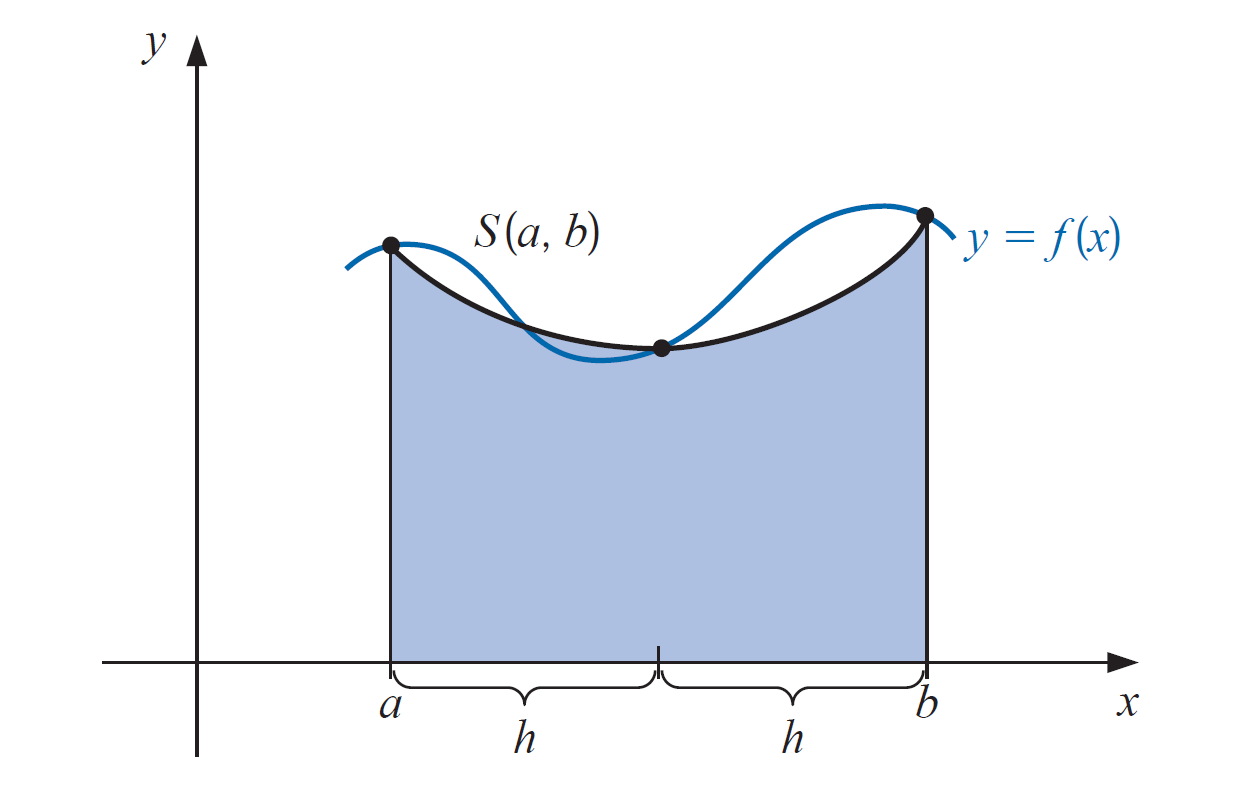
\includegraphics[scale=0.325]{pas1_cuad_ad}
\end{minipage} \\

\begin{minipage}{0.65\textwidth}
    \textbf{Al doilea pas} este sa \textit{injumatatim} intervalul $[a,b]$
    
    Astfel, obtinem punctul din mijloc \framebox{$c = \frac{a+b}{2}$} \\
    
    Atunci, $I(f)[a,b] = I(f)[a,c] + I(f)[c,b]$
    
    Dar,
    $\begin{cases}
        I(f)[a,c] = S_1[a,c] + \textcolor{red}{E_1[a,c]} \\
        I(f)[c,b]\, = S_1[c,b] + \textcolor{red}{E_1[c,b]} \\
    \end{cases}$
    
    Notam
    $\begin{cases}
        S_2[a,b] \; \eqnot \; S_1[a,c] + S_1[c,b] \\
        \textcolor{red}{E_2[a,b]} \; \eqnot \; \textcolor{red}{E_1[a,c]} + \textcolor{red}{E_1[c,b]}
    \end{cases}$ \\
    
    Atunci,
    $I(f)[a,b] = S_2[a,b] + \textcolor{red}{E_2[a,b]}$
    
    Dar, $\textcolor{red}{E_2[a,b]} = -\frac{1}{90} \cdot (\frac{h}{2})^5 \cdot [f^{(4)}(\xi_1) + f^{(4)}(\xi_2)],\,$ 
    $\begin{cases}
        \xi_1 \in (a,c) \\
        \xi_2 \in (c,b) \\
    \end{cases}$ \\
    
    Daca $f^{(4)}$ nu se schimba mult, $\textcolor{red}{E_1[a,c]} \simeq \textcolor{red}{E_1[c,b]}$
    
    $\Rightarrow \textcolor{red}{E_2[a,b]} \simeq 2 \cdot \frac{1}{2^5} \cdot$ \textcolor{red}{$-\frac{h^5}{90} \cdot f^{(4)}(\xi)$}
    $\Rightarrow$
    \framebox{$\textcolor{red}{E_2[a,b]} \simeq \frac{1}{2^4} \cdot \textcolor{red}{E_1[a,b]}$} \\
    
    Reamintim faptul ca
    $\begin{cases}
        \textcolor{red}{E_2[a,b]} \equiv \; $eroarea cu pas $ \frac{h}{2} \\
        \textcolor{red}{E_1[a,b]} \equiv \; $eroarea cu pas $ h \\
    \end{cases}$
\end{minipage}\hspace{-0.475cm}
\begin{minipage}{0.6\textwidth}
    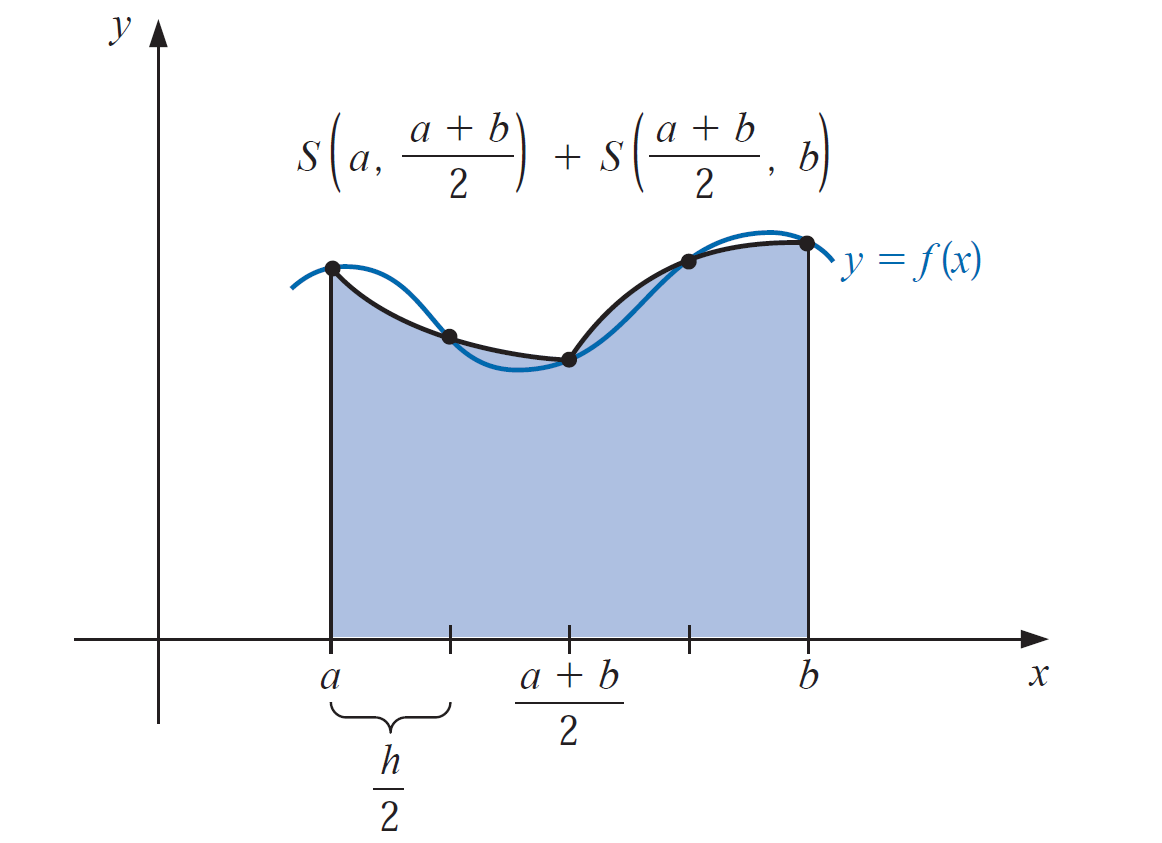
\includegraphics[scale=0.35]{pas2_cuad_ad}
\end{minipage} \\\\



\textbf{Concluzionand}, daca integram pe tot intrevalul $[a,b]$, obtinem:\, $I(f) = S_1 + \textcolor{red}{E_1}$, iar daca integram cu punctul $c$ la mijloc, obtinem: $I(f) = S_2 + \textcolor{red}{E_2}$, unde $\textcolor{red}{E_2} = \frac{1}{2^4} \cdot \textcolor{red}{E_1}$ 

Egaland cele $2$ ecuatii, obtinem: $S_2 - S_1 = 15 \textcolor{red}{E_2}$. Asadar, putem aproxima \framebox{$\textcolor{red}{E_2} = \frac{1}{15} \cdot (S_2 - S_1)$}

Asta inseamna ca aproximatia cu pas $\frac{h}{2}$ este de $15$ ori mai buna decat aproximatia cu pas~$h$. 

Reamintim faptul ca
$\begin{cases}
    S_2 \equiv \; $aproximatia Simpson cu pas $ \frac{h}{2} \\
    S_1 \equiv \; $aproximatia Simpson cu pas $ h \\
\end{cases}$ 

Deci, cand $f^{(4)}$ NU variaza mult, putem aproxima \framebox{$I = S_2 + \frac{S_2 - S_1}{15}$}

Practic, aproximam si eroarea $\textcolor{red}{E_2}$, astfel ne apropiem mult mai repede de rezultatul dorit. 

\subsubsection{Pseudocod}

\tabto{0.5cm} $function\, [S] = adaptive\_simpson(f, st, dr, tol)$
    \tabto{1cm} $mij = st + \frac{dr-st}{2}$ (echivalent cu: $\frac{st+dr}{2}$) \framebox[0.4cm][r]{\footnotemark}
    \footnotetext{\framebox[16.6cm]{\url{https://cs.stackexchange.com/questions/80415/why-is-binary-search-using-this-weird-thing-to-calculate-middle}}}
    \tabto{1cm} Compute S1 = Simpson pe $[st,dr]$
    \tabto{1cm} Compute S2 = Simpson pe $[st,mij]$ + Simpson pe $[mij,dr]$ \\

    \tabto{1cm} \textit{Daca} $|S_2 - S_1| < 15 \cdot tol$ (functia $f^{(4)}$ nu se schimba mult)
        \tabto{1.5cm} $S = S_2 + \frac{S_2 - S_1}{15}$\vspace{0.1cm}
        
    \tabto{1cm} \textit{Altfel} (functia $f^{(4)}$ variaza mult)
        \tabto{1.5cm} $mij = st + \frac{dr-st}{2}$
        \tabto{1.5cm} $left = adaptive\_simpson(f, st, mij, \frac{tol}{2})$
        \tabto{1.5cm} $right = adaptive\_simpson(f, mij, dr, \frac{tol}{2})$
        \tabto{1.5cm} $S = left + right$ 
\tabto{0.5cm} $endfunction$ \\


\tabto{0.5cm} \textit{Observatie:} Se apeleaza recursiv \textit{left} si \textit{right} cu tolerantele $\frac{tol}{2}$ pentru ca suma lor va avea cu siguranta o toleranta mai mica decat \textit{tol}.


\subsubsection{Animatie}

\tab Foarte utila in intelegerea modului de lucru al algoritmului, 
este urmatoarea \framebox{\href{https://imgur.com/a/Nr8fsxs}{Animatie}} \newpage

\subsection{Rezumat formule integrare}
% Cheatsheet
\begin{mdframe16cm}
    \vspace{0.25cm}\tabto{0.5cm}\textbf{Regula Simpla a Trapezelor (*)}\\
    
    \tabto{1cm}\framebox{$\int_a^b f(x)\, dx \simeq \frac{h}{2} [f(a) + f(b)]$} ($h=b-a$)\\
    
    \tabto{0.5cm}\textbf{Regula Compusa a Trapezelor (**)}\\
    
    \tabto{1cm}\framebox{$\int_a^b f(x)\, dx \simeq h \cdot [\frac{f(x_0) + f(x_n)}{2} + \sum\limits_{i=1}^{n-1} f(x_i)] \; \eqnot \; T(f;h)$}, $h = \frac{b-a}{n}$\\
    
    \tabto{0.5cm}\textbf{Regula Simpla Simpson (***)}\\
    
    \tabto{1cm}\framebox{$\int_a^b f(x)\, dx \simeq \frac{h}{3} \cdot [f(a) + 4f(\frac{a+b}{2}) + f(b)]$}, $h = \frac{b-a}{2}$\\
    
    \tabto{0.5cm}\textbf{Regula Compusa Simpson (****)}
    \tabto{1cm}\framebox{$\int_a^b f(x)\, dx \simeq \frac{h}{3} \cdot [f(x_0) + f(x_{2n}) + 4 \cdot \sum\limits_{i=1}^{n} f(x_{2i-1}) + 2 \cdot \sum\limits_{i=1}^{n-1} f(x_{2i})] \; \eqnot \; S(f;h)$}, $h = \frac{b-a}{2n}$
\end{mdframe16cm}


\section{Probleme Propuse}
\label{sec:probleme}

%New colors defined below
\definecolor{codegreen}{rgb}{0,0.6,0}
\definecolor{codegray}{rgb}{0.5,0.5,0.5}
\definecolor{codepurple}{rgb}{0.58,0,0.82}
\definecolor{backcolour}{rgb}{0.95,0.95,0.92}

%Code listing style named "mystyle"
\lstdefinestyle{mystyle}{
  backgroundcolor=\color{backcolour},   commentstyle=\color{codegreen},
  keywordstyle=\color{magenta},
  numberstyle=\tiny\color{codegray},
  stringstyle=\color{codepurple},
  basicstyle=\ttfamily\footnotesize,
  breakatwhitespace=false,         
  breaklines=true,                 
  captionpos=b,                    
  keepspaces=true,                 
  numbers=left,                    
  numbersep=5pt,                  
  showspaces=false,                
  showstringspaces=false,
  showtabs=false,                  
  tabsize=2,
  showlines=true,
}

%"mystyle" code listing set
\lstset{style=mystyle}

\subsection{Problema 1 - Derivata I}
\tab Completati urmatoarele programe Octave pentru a calcula \textbf{derivatele I} ale functiilor in punctele de interes.\\
\tabto{0.5cm} Descarca scriptul:
\href{https://github.com/Iulian277/Numerical-Differentiation-and-Integration/blob/main/Derivare/Prima\%20derivata/TwoPoints.m}{
\includegraphics[scale=0.35]{download_button}}
\lstinputlisting[firstline=1, lastline=12, language=Octave]{src/TwoPoints.m}
\tabto{0.5cm} Descarca scriptul:
\href{https://github.com/Iulian277/Numerical-Differentiation-and-Integration/blob/main/Derivare/Prima\%20derivata/ThreePoints_Mid.m}{
\includegraphics[scale=0.35]{download_button}}
\lstinputlisting[firstline=1, lastline=12, language=Octave]{src/ThreePoints_Mid.m}
\tabto{0.5cm} Descarca scriptul:
\href{https://github.com/Iulian277/Numerical-Differentiation-and-Integration/blob/main/Derivare/Prima\%20derivata/ThreePoints_End.m}{
\includegraphics[scale=0.35]{download_button}}
\lstinputlisting[firstline=1, lastline=11, language=Octave]{src/ThreePoints_End.m}

Pentru testarea programelor, puteti folosi urmatoarea functie:\\
\tabto{0.5cm} Descarca scriptul:
\href{https://github.com/Iulian277/Numerical-Differentiation-and-Integration/blob/main/Derivare/Prima\%20derivata/testare_derivate.m}{
\includegraphics[scale=0.35]{download_button}}
\lstinputlisting[firstline=1, lastline=13, language=Octave]{src/testare_derivate.m} \vspace{0.5cm}


\subsection{Problema 2 - Derivata II}
\tab Completati urmatoarea functie Octave pentru a calcula \textbf{derivatele II} ale functiilor in punctele de interes.\\
\tabto{0.5cm} Descarca scriptul:
\href{https://github.com/Iulian277/Numerical-Differentiation-and-Integration/blob/main/Derivare/A\%20doua\%20derivata/ThreePoints.m}{
\includegraphics[scale=0.35]{download_button}}
\lstinputlisting[firstline=1, lastline=10, language=Octave]{src/ThreePoints.m}

Pentru testarea programului, puteti folosi urmatoarea functie:\\
\tabto{0.5cm} Descarca scriptul:
\href{https://github.com/Iulian277/Numerical-Differentiation-and-Integration/blob/main/Derivare/A\%20doua\%20derivata/testare_derivate.m}{
\includegraphics[scale=0.35]{download_button}}
\lstinputlisting[firstline=1, lastline=11, language=Octave]{src/testare_derivate2.m} \vspace{0.5cm}


\subsection{Problema 3 - Integrare}
\tab Completati urmatoarele functii Octave pentru a calcula \textbf{integralele definite} ale functiilor pe intervalele de interes.\\
\tabto{0.5cm} Descarca scriptul:
\href{https://github.com/Iulian277/Numerical-Differentiation-and-Integration/blob/main/Integrare/Newton-Cotes/trapez_simplu.m}{
\includegraphics[scale=0.35]{download_button}}
\lstinputlisting[firstline=1, lastline=16, language=Octave]{src/trapez_simplu.m} \newpage

\tabto{0.5cm} Descarca scriptul:
\href{https://github.com/Iulian277/Numerical-Differentiation-and-Integration/blob/main/Integrare/Newton-Cotes/trapez_compus.m}{
\includegraphics[scale=0.35]{download_button}}
\lstinputlisting[firstline=1, lastline=17, language=Octave]{src/trapez_compus.m}

\tabto{0.5cm} Descarca scriptul:
\href{https://github.com/Iulian277/Numerical-Differentiation-and-Integration/blob/main/Integrare/Newton-Cotes/Simpson_simplu.m}{
\includegraphics[scale=0.35]{download_button}}
\lstinputlisting[firstline=1, lastline=16, language=Octave]{src/Simpson_simplu.m}

\tabto{0.5cm} Descarca scriptul:
\href{https://github.com/Iulian277/Numerical-Differentiation-and-Integration/blob/main/Integrare/Newton-Cotes/Simpson_compus.m}{
\includegraphics[scale=0.35]{download_button}}
\lstinputlisting[firstline=1, lastline=17, language=Octave]{src/Simpson_compus.m}

Pentru testarea programului, puteti folosi urmatoarea functie:\\
\tabto{0.5cm} Descarca scriptul:
\href{https://github.com/Iulian277/Numerical-Differentiation-and-Integration/blob/main/Integrare/Newton-Cotes/testare_Newton_Cotes.m}{
\includegraphics[scale=0.35]{download_button}}
\lstinputlisting[firstline=1, lastline=13, language=Octave]{src/testare_Newton_Cotes.m}

Pentru testarea programului, veti avea nevoie si de functia care aplica interpolarea Lagrange pe un set de puncte (vezi \textit{Laborator Interpolare}).
\tabto{0.5cm} Descarca scriptul:
\href{https://github.com/Iulian277/Numerical-Differentiation-and-Integration/blob/main/Integrare/Newton-Cotes/lagrange.m}{
\includegraphics[scale=0.35]{download_button}}
\lstinputlisting[firstline=1, lastline=7, language=Octave]{src/lagrange.m}


\subsection{Extra}
\tab In incheiere, puteti lectura un material referitor la utilizarea integrarii numerice intr-o aplicatie din viata reala (\textbf{Reverse Osmosis Model}): \href{https://github.com/Iulian277/Numerical-Differentiation-and-Integration/blob/main/Reverse_Osmosis_Model_Integration.pdf}{
\includegraphics[scale=0.4]{document_button}}


\end{document}
